% ===================================================================
% LaTeX Template for MATH 0290 Project Report
% ===================================================================

\documentclass[12pt, a4paper]{article}

\usepackage[utf8]{inputenc}

% --- 核心宏包 (Essential Packages) ---

% 数学公式支持 (for math formulas, matrices, etc.)
\usepackage{amsmath}
\usepackage{amssymb}
\usepackage{amsthm}
\usepackage{tikz}
\usetikzlibrary{arrows.meta, positioning, shapes.geometric}
% 页面边距设置 (for setting margins)
\usepackage[margin=1in]{geometry}

% 插入图片支持 (for including plots from Python/MATLAB)
\usepackage{graphicx}
\usepackage{float}

% 超链接支持 (makes PDF interactive, e.g., clickable ToC)
\usepackage{hyperref}

% 设置段落缩进和间距 (for paragraph formatting)
\usepackage{indentfirst}
\setlength{\parskip}{0.5em}

% --- 美化宏包与设置 (Aesthetic Packages & Settings) ---

% 颜色支持
\usepackage{xcolor}
% 使用更现代的字体
\usepackage{lmodern}
% 用于页眉页脚
\usepackage{fancyhdr}
% 用于定制章节标题
\usepackage{titlesec}
% 用于定制图表标题
\usepackage{caption}

% 重新定义 abstract 环境以匹配正文字体大小和边距
\renewenvironment{abstract}
 {\normalsize
  \begin{center}
  \bfseries \abstractname
  \end{center}
  \list{}{\setlength{\leftmargin}{0em}\setlength{\rightmargin}{\leftmargin}}%
  \item\relax}
 {\endlist}

% 定义主题颜色
\definecolor{primarycolor}{rgb}{0.12, 0.3, 0.53} % A professional blue

% 调整超链接颜色以保持一致性
\hypersetup{
    colorlinks=true,
    linkcolor=primarycolor,
    filecolor=magenta,      
    urlcolor=cyan,
    citecolor=green!60!black,
}

% 页眉页脚设置
\pagestyle{fancy}
\fancyhf{} % 清空所有页眉页脚
\fancyhead[L]{\leftmark} % 左侧页眉显示章节名称
\fancyfoot[C]{\thepage} % 页面底部中央显示页码
\renewcommand{\headrulewidth}{0.4pt}
\renewcommand{\footrulewidth}{0pt} % 通常页脚线不是必需的
% 为像目录页这样的普通页面设置样式
\fancypagestyle{plain}{%
  \fancyhf{}%
  \fancyfoot[C]{\thepage}%
  \renewcommand{\headrulewidth}{0pt}%
  \renewcommand{\footrulewidth}{0pt}%
}

% 章节标题格式设置
\titleformat{\section}
  {\normalfont\Large\bfseries\color{primarycolor}}
  {\thesection}
  {1em}
  {}
  [\color{primarycolor!40}\titlerule]

\titleformat{\subsection}
  {\normalfont\large\bfseries\color{primarycolor!90!black}}
  {\thesubsection}
  {1em}
  {}

\titleformat{\subsubsection}
  {\normalfont\normalsize\bfseries\color{black}}
  {\thesubsubsection}
  {1em}
  {}

% 图表标题格式设置 (Figure and Table captions)
\captionsetup{
    labelfont={bf, color=primarycolor},
    labelsep=period,
    justification=centering,
    singlelinecheck=false
}

% 新增:用于代码清单的宏包
\usepackage{listings}

% 设置代码清单样式
\definecolor{codegreen}{rgb}{0,0.6,0}
\definecolor{codegray}{rgb}{0.5,0.5,0.5}
\definecolor{codepurple}{rgb}{0.58,0,0.82}
\definecolor{backcolour}{rgb}{0.95,0.95,0.92}

    \lstdefinestyle{mystyle}{
        backgroundcolor=\color{backcolour},   
        commentstyle=\color{codegreen},
        keywordstyle=\color{magenta},
        numberstyle=\tiny\color{codegray},
        stringstyle=\color{codepurple},
        basicstyle=\ttfamily\footnotesize,
        breakatwhitespace=false,         
        breaklines=true,                 
        captionpos=b,                    
        keepspaces=true,                 
        numbers=left,                    
        numbersep=5pt,                  
        showspaces=false,                
        showstringspaces=false,
        showtabs=false,                  
        tabsize=2,
        literate={β}{{$\beta$}}1 {ρ}{{$\rho$}}1,
        mathescape=true
    }
\lstset{style=mystyle}


% ===================================================================
%   文档开始 (Document Begins)
% ===================================================================

\begin{document}

% --- 标题部分 (Title Block) ---
\begin{titlepage}
    \begin{tikzpicture}[remember picture, overlay]
        % 创建顶部的蓝色标题栏
        \node[yshift=-4.5cm] at (current page.north) [rectangle, fill=primarycolor, anchor=north, minimum width=\paperwidth, minimum height=7cm]{};
        
        % 在标题栏内放置白色标题文本
        \node[yshift=-8cm, text=white] at (current page.north) [text width=0.9\textwidth, align=center] {
            \huge\bfseries Bayesian Inference of a Piecewise SEIAR Model \\[0.5em]
            \huge\bfseries for COVID-19 Dynamics
        };
    \end{tikzpicture}
    
    \centering
    
    % 1. 使用固定间距将所有内容推到标题栏下方
    \vspace*{12cm} 
    
    % 2. 作者信息模块
    {\Large\bfseries Axel Young\par}
    \vspace{1em}
    {\large Student ID: 2023141520034\par}
    \vspace{1em}
    {\large\href{https://github.com/AxelYoung/DE_Project}{GitHub Repository: github.com/AxelYoung/DE\_Project}\par}

    % 3. 使用 \vfill 在模块间创建动态的、相等的间距
    \vfill
    
    % 4. 课程与导师信息模块
    {\large A Project for the course\par}
    \vspace{0.5em}
    {\large\bfseries Differential Equations\par}
    \vspace{1.5em}
    {\large Submitted to\par}
    \vspace{0.5em}
    {\large\bfseries Prof. Peng Zeng\par}
    
    \vfill

    % 5. 日期模块
    {\Large \today\par}
    
    % 在页面底部留出一些空白
    \vspace*{2cm}

\end{titlepage}

% --- 摘要 (Abstract) ---
\begin{abstract}
    This report investigates the transmission dynamics of the COVID-19 epidemic in Germany by developing and calibrating a compartmental model. Beginning with the foundational Susceptible-Infectious-Recovered (SIR) model, this project progresses to a more sophisticated Susceptible-Exposed-Infectious-Asymptomatic-Recovered (SEIAR) framework to account for key real-world features such as latent periods and asymptomatic transmission. We detail the iterative process of model calibration, starting with a deterministic least-squares fit and advancing to a full Bayesian inference model with piecewise parameters to capture the dynamic impact of public health interventions. The calibrated model is then used to conduct scenario analysis, quantifying the effectiveness of measures aimed at reducing transmission rates. The findings demonstrate that a multi-stage Bayesian model can accurately describe complex epidemic trajectories and provide valuable, data-driven insights for public health policy, while also highlighting the limitations of simplified modeling assumptions.
\end{abstract}
\clearpage
% --- 目录 (Table of Contents) ---
\tableofcontents
\newpage

% --- 报告正文 (Report Body) ---

\section{Introduction}
The spread of infectious diseases represents a significant and persistent threat to global public health and economic stability. Mathematical modeling provides a powerful framework for understanding these complex dynamics and is a critical step toward the development of effective strategies for public health intervention. This project utilizes systems of first-order ordinary differential equations (ODEs) to model and analyze the propagation of an epidemic through a population, thereby connecting core mathematical concepts to real-world epidemiological challenges.

The analysis will begin with the foundational Susceptible-Infectious-Recovered (SIR) model, which serves as a baseline for more complex investigations. The governing equations of the SIR model will be derived and its dynamic properties, including equilibrium points and stability, will be thoroughly analyzed. Following this, the model will be extended to incorporate more realistic scenarios, such as demographic changes within the population. To ground the theoretical framework in reality, the extended model will be validated against real-world disease data, from which key transmission parameters will be estimated. Finally, the report will present simulations under various conditions and conclude with a critical discussion of the model's underlying assumptions, its inherent limitations, and its practical applications in shaping public health policy.

\section{Part 1: Foundations of the SIR Model}
Many early epidemiological models were devoted to mathematical modeling at the population level, assuming various kinds of homogeneity. The simplest and most foundational of these is the Susceptible-Infectious-Recovered (SIR) model, first described by Kermack and McKendrick (1927) for a closed population. It provides a deterministic framework for understanding the core dynamics of an epidemic.

\subsection{The Model Compartments}
The model is based on a compartmentalization of the total population ($N$) into three distinct epidemiological states. This structure is consistent with the classic framework described in the reference literature. The compartments are:

\begin{itemize}
    \item \textbf{Susceptible (S):} Individuals who are healthy but can be infected upon contact with the pathogen.
    \item \textbf{Infectious (I):} Individuals who are currently infected and are capable of transmitting the disease to susceptible individuals.
    \item \textbf{Recovered (R):} Individuals who have been removed from the infection cycle, either through recovery and subsequent immunity, or through death.
\end{itemize}

The model assumes a constant total population, such that $S(t) + I(t) + R(t) = N$.

\subsection{Model Dynamics and Governing Equations}
The transmission dynamics are represented by the flow of individuals between these compartments: $S \to I \to R$. This process is captured by a system of ordinary differential equations (ODEs).

\subsubsection{Rate of Change of the Susceptible Population ($\frac{dS}{dt}$)}
This rate is determined by the incidence of new infections. Assuming a homogeneously mixing population, the number of interactions between susceptible and infectious individuals is proportional to their product, $SI$. If we let $\beta$ be the transmission rate, representing the probability of disease transmission per contact multiplied by the contact rate, then the rate of new infections is $\beta SI$. Since this flow removes individuals from the susceptible class, the equation is:
\begin{equation} \label{eq:dSdt}
\frac{dS}{dt} = -\beta SI
\end{equation}

\subsubsection{Rate of Change of the Infectious Population ($\frac{dI}{dt}$)}
The infectious population is increased by the newly infected individuals from the susceptible class (at a rate of $+\beta SI$) and decreased by individuals who recover. Assuming that a constant fraction, $g$, of the infectious population recovers per unit of time, the rate of recovery is $gI$. Therefore, the net change is:
\begin{equation} \label{eq:dIdt}
\frac{dI}{dt} = \beta SI - gI
\end{equation}

\subsubsection{Rate of Change of the Recovered Population ($\frac{dR}{dt}$)}
The recovered population only increases as individuals from the infectious class recover. The rate of this flow is therefore:
\begin{equation} \label{eq:dRdt}
\frac{dR}{dt} = gI
\end{equation}

This system of equations~(\ref{eq:dSdt})--(\ref{eq:dRdt}) aligns with the bilinear incidence formulation provided in the project brief.


\subsection{Model Parameters}
The model's behavior is dictated by two key parameters:

\begin{description}
    \item[$\beta$ (Transmission Rate)] This coefficient represents the effective contact rate leading to infection. As described in the reference literature, it can be considered the product of the average number of contacts per unit time and the probability of infection given a contact between an infectious and a susceptible individual.
    \item[$g$ (Recovery Rate, often denoted as $\gamma$)] This parameter represents the per capita rate of recovery for infectious individuals. The reciprocal, $1/g$, is interpreted as the average duration of the infectious period.
\end{description}

\subsection{Key Assumptions and Limitations}
The simplicity and analytical tractability of the SIR model are based on several key assumptions. As noted in the reference literature, these assumptions provide a foundation but also introduce limitations:

\begin{itemize}
    \item \textbf{Homogeneous Mixing:} The model assumes that all individuals in the population have an equal chance of interacting with one another, and it is "not designed to capture details of individual connection patterns and networks".
    \item \textbf{Continuous and Homogeneous Population:} The population is treated as a continuous entity, not as discrete individuals, and parameters like $\beta$ and $g$ are assumed to be uniform across all individuals, ignoring variations due to age, behavior, or genetics.
    \item \textbf{Closed Population \& Permanent Immunity:} The model assumes a closed population with no births or deaths and that recovery confers lifelong immunity (SIS models are used when immunity wanes).
\end{itemize}

These assumptions are critical for providing a simplified, solvable system, but they also constrain the model's direct applicability to complex real-world epidemics. These limitations will be addressed in subsequent sections through model extensions and critical analysis.

This section establishes the theoretical foundation of the SIR model, which is essential for the subsequent analysis of equilibrium points and stability.

\subsection{Equilibrium Points and Stability Analysis}
The stability of the system is analyzed at its equilibrium points, which are the steady states where all rates of change are zero. The Jacobian matrix is derived from the core dynamics of the susceptible ($S$) and infectious ($I$) populations, since the recovered ($R$) population does not feed back into the other two. The matrix for the system is:
\[
J(S,I) =
\begin{pmatrix}
    -\beta I & -\beta S \\
    \beta I  & \beta S - g
\end{pmatrix}
\]
The stability is determined by the eigenvalues of this matrix evaluated at the system's equilibrium points.

\subsubsection{The Disease-Free Equilibrium (DFE)}
The disease-free equilibrium (DFE) represents the state where the infection is absent from the population, defined by $I=0$. Substituting $I=0$ into the SIR system equations yields $\frac{dS}{dt} = 0$ and $\frac{dI}{dt} = 0$. In a closed population of size $N$ with no prior immunity, this corresponds to the state where the entire population is susceptible. Thus, the DFE point, denoted $E_0$, is:
\[ E_0 = (S,I) = (N,0) \]

\subsubsection{Stability of the DFE}
To analyze the stability of the DFE, we evaluate the Jacobian matrix at the point $E_0 = (N,0)$:
\[
J(N,0) =
\begin{pmatrix}
    -\beta(0) & -\beta N \\
    \beta(0)  & \beta N - g
\end{pmatrix}
=
\begin{pmatrix}
    0 & -\beta N \\
    0 & \beta N - g
\end{pmatrix}
\]
As this is an upper-triangular matrix, its eigenvalues are the elements on the main diagonal. The eigenvalues ($\lambda$) of the system at the DFE are therefore:
\[ \lambda_1 = 0 \quad \text{and} \quad \lambda_2 = \beta N - g \]
For the DFE to be stable, the real parts of all eigenvalues must be negative. The eigenvalue $\lambda_1 = 0$ is a neutral eigenvalue related to the conservation of the total population, so the stability of the system with respect to the introduction of the disease is determined by the sign of $\lambda_2$.

The condition for stability is $\lambda_2 < 0$, which implies:
\[ \beta N - g < 0 \implies \frac{\beta N}{g} < 1 \]
This ratio is the critically important Basic Reproduction Number ($R_0$), which represents the average number of secondary infections produced by a single infectious individual in a completely susceptible population. We define it as:
\[ R_0 = \frac{\beta N}{g} \]
Therefore, the disease-free equilibrium is locally asymptotically stable if and only if $R_0 < 1$. In epidemiological terms, this means that if an infected individual produces, on average, less than one new infection, the disease will fail to spread and will ultimately die out from the population. Conversely, if $R_0 > 1$, the DFE is unstable, and the introduction of the pathogen will lead to an epidemic outbreak.

\subsection{The Endemic Equilibrium with Vital Dynamics}
The basic SIR model assumes a closed population, which means the epidemic must eventually end as the susceptible population is depleted. To analyze the long-term persistence of a disease—its \textit{endemic state}—we must consider population turnover. Following a key extension mentioned in the project brief, we introduce births and deaths, both occurring at an equal rate $\mu$, keeping the total population $N$ constant. The governing equations are:
\begin{align}
    \frac{dS}{dt} &= \mu N - \beta SI - \mu S \\
    \frac{dI}{dt} &= \beta SI - (\gamma + \mu)I \\
    \frac{dR}{dt} &= \gamma I - \mu R
\end{align}
An endemic equilibrium (EE) is a steady state where the disease persists in the population, i.e., $I^* > 0$. To find this equilibrium, we set the derivatives to zero. From the equation for $\frac{dI}{dt}$, we have $I(\beta S - (\gamma + \mu)) = 0$. Since we are looking for a state where $I \neq 0$, it must be that:
\[ S^* = \frac{\gamma + \mu}{\beta} \]
Substituting this into the equation for $\frac{dS}{dt}$ and setting it to zero allows us to solve for $I^*$:
\[ \mu N - \beta S^* I^* - \mu S^* = 0 \implies I^* = \frac{\mu(N - S^*)}{\beta S^*} = \frac{\mu(N - \frac{\gamma + \mu}{\beta})}{\gamma + \mu} = \frac{\mu N}{\gamma + \mu} - \frac{\mu}{\beta} \]
This endemic equilibrium is biologically meaningful only if $I^* > 0$. This condition requires:
\[ \frac{\mu N}{\gamma + \mu} > \frac{\mu}{\beta} \implies \frac{\beta N}{\gamma + \mu} > 1 \]
The term on the left is the basic reproduction number for this model with vital dynamics, often written as $R_0 = \frac{\beta N}{\gamma + \mu}$. Therefore, a stable endemic equilibrium is possible if and only if $R_0 > 1$. This analysis directly addresses the project requirement to investigate endemic states and demonstrates that for a disease to become endemic, each infected individual must, on average, produce more than one new infection to counteract both recovery and removal from the population via death.

\section{Part 2: Extended Model with Asymptomatic Transmission}
The basic SIR model provides a valuable but simplified view of an epidemic. Its assumptions, such as immediate infectiousness upon infection and a uniform infectious class, limit its applicability to complex diseases like COVID-19. Key real-world features are not captured, including the latent (or exposed) period where an individual is infected but not yet infectious~\cite{Wong2020}, and the significant role of asymptomatic transmission, where individuals spread the virus without ever showing clinical symptoms~\cite{Byambasuren2020}. To build a more robust and realistic framework, we extend the foundational SIR model to an SEIAR (Susceptible-Exposed-Infectious-Asymptomatic-Recovered) model.

\subsection{The SEIAR Model Compartments and Flow}
The total population ($N$) is now partitioned into five distinct compartments:
\begin{itemize}
    \item \textbf{S (Susceptible):} Individuals who can contract the disease.
    \item \textbf{E (Exposed):} Individuals who have been infected but are in the incubation period and not yet capable of transmitting the virus.
    \item \textbf{I (Symptomatic Infectious):} Individuals who are infectious and exhibit clinical symptoms.
    \item \textbf{A (Asymptomatic Infectious):} Individuals who are infectious but do not show any clinical symptoms throughout their illness.
    \item \textbf{R (Recovered):} Individuals who are assumed to have permanent immunity.
\end{itemize}
The flow of individuals through the compartments is more complex than in the SIR model. A susceptible individual who becomes infected first enters the exposed class. After the latent period, this individual can then become either symptomatically or asymptomatically infectious, before eventually moving to the recovered class. The model structure is illustrated in Figure~\ref{fig:seiar_flow_part2}.

\begin{figure}[h!]
\centering
\begin{tikzpicture}[
node distance=2.5cm and 2cm,
box/.style={rectangle, draw, thick, text centered, minimum height=1cm, minimum width=2cm},
arrow/.style={-Latex, thick}
]

    \node[box] (S) {Susceptible (S)};
    \node[box, right=of S] (E) {Exposed (E)};
    \node[box, above right=of E] (I) {Infectious (I)};
    \node[box, below right=of E] (A) {Asymptomatic (A)};
    \node[box, right=of I, xshift=1cm] (R) {Recovered (R)};
    
    \draw[arrow] (S) -- node[above] {} (E);
    \draw[arrow] (E.north) -- ++(0,0.5cm) -| node[above, near start] {$(1-f)\sigma$} (I.west);
    \draw[arrow] (E.south) -- ++(0,-0.5cm) -| node[below, near start] {$f\sigma$} (A.west);
    \draw[arrow] (I) -- node[above] {$\gamma_I$} (R);
    \draw[arrow] (A) -- node[below] {$\gamma_A$} (R);

\end{tikzpicture}
\caption{Flow diagram of the SEIAR (Susceptible-Exposed-Infectious-Asymptomatic-Recovered) model structure. A fraction, $f$, of exposed individuals becomes asymptomatic, while the fraction $(1-f)$ becomes symptomatic.}
\label{fig:seiar_flow_part2}
\end{figure}

\subsection{Governing Equations of the SEIAR Model}
The dynamics of the SEIAR model are described by the following system of five ordinary differential equations:
\begin{align}
\frac{dS}{dt} &= -\beta_I SI - \beta_A SA \\
\frac{dE}{dt} &= \beta_I SI + \beta_A SA - \sigma E \\
\frac{dI}{dt} &= (1-f)\sigma E - \gamma_I I \\
\frac{dA}{dt} &= f\sigma E - \gamma_A A \\
\frac{dR}{dt} &= \gamma_I I + \gamma_A A
\end{align}

\subsection{Parameters for the Extended Model}
The parameters for this extended model are established based on a review of current epidemiological literature for COVID-19. The key structural parameters, their meanings, and their data-supported values are summarized in Table~\ref{tab:params}. The primary transmission rate, $\beta_I$, remains to be estimated from data in Part 3.

\begin{table}[h!]
\centering
\caption{Parameters for the Extended SEIAR Model based on COVID-19 Literature}
\begin{tabular}{|c|l|l|l|}
\hline
\textbf{Symbol} & \textbf{Parameter} & \textbf{Value / Relationship} & \textbf{Source} \\
\hline
$f$ & Asymptomatic Proportion & $\approx 0.17$ (17\%) & \cite{Byambasuren2020} \\
$\beta_A / \beta_I$ & Relative Infectiousness & 0.58 & \cite{Byambasuren2020} \\
$1/\sigma$ & Mean Incubation Period & 4.5 days & \cite{Wong2020} \\
$1/\gamma_I$ & Symptomatic Infectious Period & 19.5 days & \cite{Wang2022} \\
$1/\gamma_A$ & Asymptomatic Infectious Period & 17.0 days & \cite{Wang2022} \\
\hline
$\beta_I$ & Transmission Rate (Symptomatic) & To be estimated & - \\
\hline
\end{tabular}
\label{tab:params}
\end{table}

This SEIAR framework provides a more nuanced and realistic foundation for modeling the epidemic. The subsequent task is to analyze its mathematical properties, specifically its equilibrium states and the conditions for an outbreak, which will now depend on this more complex set of interactions and parameters.

\subsection{Mathematical Analysis of the SEIAR Model}
To analyze the stability of the SEIAR model's DFE, we must determine the sign of the eigenvalues of its Jacobian matrix. However, with three infected compartments (E, I, A), this would require analyzing a large and algebraically intensive 4x4 matrix. The Next-Generation Matrix (NGM) method~\cite{vandenDriessche2002} offers a more systematic and powerful approach to derive the threshold condition, $R_0$, for such multi-compartment systems. This method focuses on the dynamics within the infected compartments to calculate the threshold for epidemic invasion.

\subsubsection{The Disease-Free Equilibrium}
The DFE for the SEIAR model is the state where there are no individuals in any of the infected compartments, i.e., $E=0, I=0$, and $A=0$. In a closed population of size $N$, this corresponds to the state where the entire population is susceptible. The DFE, denoted $E_0$, is therefore:
\[ E_0 = (S,E,I,A) = (N,0,0,0) \]

\subsubsection{The Next-Generation Matrix Method}
The NGM method separates the rates of change in the infected compartments into two components: the rate of new infections ($\mathcal{F}$) and the rates of all other transitions between compartments ($\mathcal{V}$). For our model, the infected compartments are E, I, and A. The corresponding equations are:
\begin{align*}
\frac{dE}{dt} &= (\beta_I SI + \beta_A SA) - \sigma E \\
\frac{dI}{dt} &= (1-f)\sigma E - \gamma_I I \\
\frac{dA}{dt} &= f\sigma E - \gamma_A A
\end{align*}
From these, we construct the matrices $F$ (the Jacobian of new infection terms) and $V$ (the Jacobian of transition terms), evaluated at the DFE ($S=N, I=0, A=0$).

The matrix of new infection rates, $F$, is:
\[
F = \begin{pmatrix}
0 & \beta_I N & \beta_A N \\
0 & 0 & 0 \\
0 & 0 & 0
\end{pmatrix}
\]
The matrix of transition rates, $V$, is:
\[
V = \begin{pmatrix}
\sigma & 0 & 0 \\
-(1-f)\sigma & \gamma_I & 0 \\
-f\sigma & 0 & \gamma_A
\end{pmatrix}
\]

\subsubsection{Derivation of the Basic Reproduction Number ($R_0$)}
The Basic Reproduction Number is given by the spectral radius (largest eigenvalue) of the next-generation matrix, $K = FV^{-1}$. First, we compute the inverse of $V$:
\[
V^{-1} = \begin{pmatrix}
1/\sigma & 0 & 0 \\
(1-f)/\gamma_I & 1/\gamma_I & 0 \\
f/\gamma_A & 0 & 1/\gamma_A
\end{pmatrix}
\]
Next, we compute the product $K = FV^{-1}$:
\[
K = 
\begin{pmatrix}
0 & \beta_I N & \beta_A N \\
0 & 0 & 0 \\
0 & 0 & 0
\end{pmatrix}
\begin{pmatrix}
1/\sigma & 0 & 0 \\
(1-f)/\gamma_I & 1/\gamma_I & 0 \\
f/\gamma_A & 0 & 1/\gamma_A
\end{pmatrix}
=
\begin{pmatrix}
 \frac{(1-f)\beta_I N}{\gamma_I} + \frac{f\beta_A N}{\gamma_A} & \frac{\beta_I N}{\gamma_I} & \frac{\beta_A N}{\gamma_A} \\
 0 & 0 & 0 \\
 0 & 0 & 0
\end{pmatrix}
\]
The eigenvalues of this matrix are its diagonal elements. The largest eigenvalue, which is the spectral radius, defines $R_0$.

Thus, for the SEIAR model, the Basic Reproduction Number is:
\[
R_0 = \frac{(1-f)\beta_I N}{\gamma_I} + \frac{f\beta_A N}{\gamma_A}
\]
The DFE is stable if $R_0 < 1$ and unstable if $R_0 > 1$. The derivation of $R_0$ is therefore equivalent to performing a stability analysis of the DFE. The condition $R_0 > 1$ implies that the largest eigenvalue of the next-generation matrix is greater than one, which in turn means the DFE is unstable and an epidemic invasion will occur.

\subsubsection{Epidemiological Interpretation of $R_0$}
This formula for $R_0$ has a clear and intuitive epidemiological interpretation. It is the sum of the number of secondary infections generated through two distinct pathways:
\begin{itemize}
    \item \textbf{The Symptomatic Pathway Contribution:} The term $\frac{(1-f)\beta_I N}{\gamma_I}$ represents the average number of new infections generated by a single primary case throughout its symptomatic phase. A primary case has a probability of $(1-f)$ of becoming symptomatic, and once symptomatic, their infectious period is $1/\gamma_I$. During this time, they cause $\beta_I N$ new infections per unit time.
    \item \textbf{The Asymptomatic Pathway Contribution:} The term $\frac{f\beta_A N}{\gamma_A}$ represents the average number of new infections generated throughout the asymptomatic phase. A primary case has a probability of $f$ of being asymptomatic, with an infectious period of $1/\gamma_A$ and a corresponding transmission rate.
\end{itemize}
The total $R_0$ for the population is the sum of the contributions from both transmission routes, reflecting the combined impact of symptomatic and asymptomatic carriers on the spread of the disease.

\section{Part 3: Data Validation and Simulation}
This section details the process of calibrating the theoretical SEIAR model developed in Part 2 against real-world epidemiological data. The objective is to estimate the unknown transmission parameters and validate the model's ability to describe the dynamics of an actual epidemic. This process was conducted in two primary phases: an initial deterministic fitting to establish a baseline, followed by a more sophisticated Bayesian inference to fully quantify parameter uncertainty and capture time-varying dynamics.

\subsection{Data Acquisition and Preprocessing}
To calibrate and validate our theoretical model against real-world phenomena, data processing is a crucial first step. This section details how we acquired, cleaned, and constructed a high-quality time-series dataset suitable for model fitting from raw data.

\paragraph{Data Source and Filtering}
As required by the project, we used the public and authoritative "Our World in Data (OWID)" dataset, provided in the \texttt{owid-covid-data.csv} file. We first loaded this global dataset using the pandas library and filtered it along two dimensions:
\begin{itemize}
    \item \textbf{Geography:} The \texttt{location} column was filtered for "Germany".
    \item \textbf{Time:} The \texttt{date} column was filtered for the period between March 1, 2020, and March 1, 2021. This window was chosen to comprehensively cover Germany's first epidemic wave and the initial phase of its second wave.
\end{itemize}

\paragraph{Data Smoothing}
The raw daily new cases data (\texttt{new\_cases}) often contains significant noise and random fluctuations caused by reporting delays (e.g., the "weekend effect"). To eliminate these disturbances and better reveal the true underlying trend of the epidemic, we applied a 7-day centered rolling average to the daily new cases. This standard data smoothing technique effectively filtered out short-term random noise, providing us with a curve, \texttt{new\_cases\_smoothed}, that more accurately reflects the true trajectory of the epidemic.

\paragraph{Constructing the Core Fitting Variable: The Infectious Pool}
The state variables I (symptomatic) and A (asymptomatic) in our SEIAR model represent the total number of currently infectious individuals at a given time (prevalence), whereas the data directly provides the number of new cases each day (incidence). This is a critical conceptual difference. To enable a meaningful comparison between the model and the data, we must estimate the daily number of existing infectious individuals from the daily new cases.

Based on findings from the literature reviewed in Part 2, the average infectious period for COVID-19 is approximately 19 days. Accordingly, we applied a 19-day rolling sum to the smoothed new cases data (\texttt{new\_cases\_smoothed}). The resulting \texttt{infectious\_pool} column represents an estimate of the total number of active, infectious cases present in the population on any given day, $t$. This time series is conceptually equivalent to the theoretical total infected population (I+A) in our model, and it therefore became the core dependent variable for all subsequent model fitting and analysis.

Through these steps, we successfully transformed the large, raw dataset into a precise, smoothed, and analysis-ready dataset, \texttt{germany\_covid\_processed.csv}, laying a solid foundation for the rigorous parameter inference that followed.

\subsection{Phase 1: Deterministic Parameter Estimation with Non-Linear Least Squares}
Our initial exploration aimed to find a single, best-fit value for the primary unknown parameter, the symptomatic transmission rate ($\beta_I$), using a rapid and intuitive method.

\subsubsection{Methodology}
We utilized the \texttt{scipy.optimize.curve\_fit} function in Python, which employs a non-linear least squares algorithm. This function seeks to find the value of $\beta_I$ that minimizes the sum of squared residuals between the output of the SEIAR model and the prepared German COVID-19 data. In this phase, all other biological parameters (e.g., $f, \sigma, \gamma_I, \gamma_A$) were held constant at the values derived from the literature review in Part 2.

\subsubsection{Iterative Strategy: The Search for a Suitable Fitting Window}
Our analysis revealed that the choice of the fitting window is decisive for the outcome. A constant $\beta_I$ cannot describe the full, year-long dynamic of an epidemic influenced by public health interventions. We therefore conducted a series of explorations to find an optimal fitting window.

\paragraph{Attempt 1: Limitation of Long-Window Fitting and Extrapolation}
We first attempted to fit the model using data from the entire first wave (first 150 days) and used the resulting $\beta_I$ to predict the subsequent six months. The result is shown in Figure \ref{fig:linear_neg1}. While the model roughly captures the shape of the first wave, its forward prediction (red line) diverges significantly from the real-world data (blue dots), demonstrating that a single $\beta_I$ is unsuited for long-term prediction in a changing environment.

\begin{figure}[h!]
    \centering
    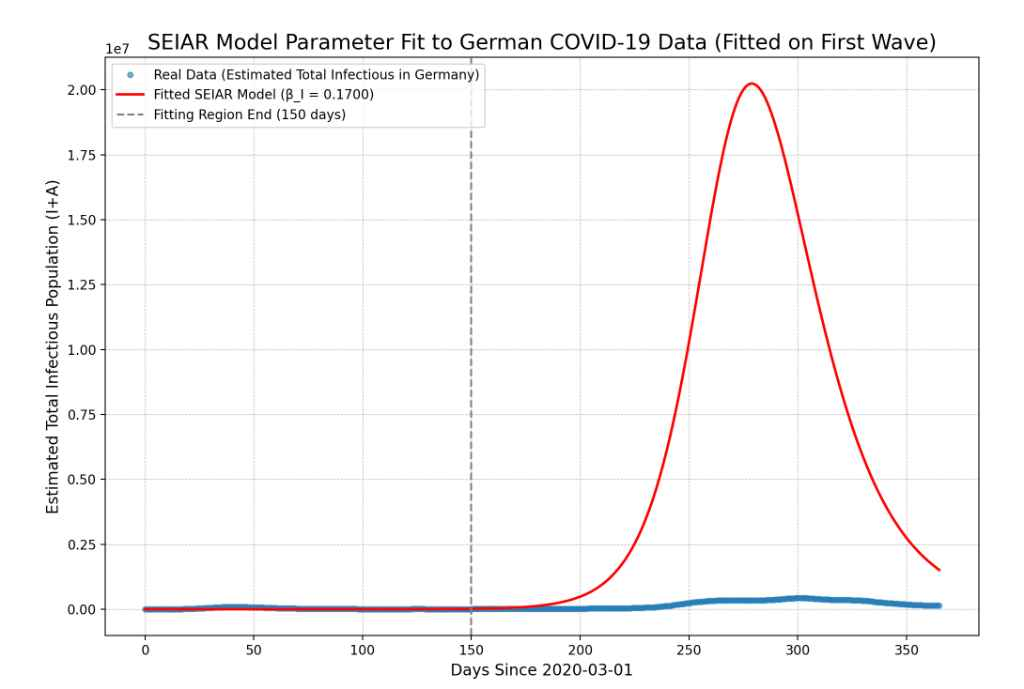
\includegraphics[width=0.8\textwidth]{1/linear_-1.png}
    \caption{Result of fitting on the first 150 days and extrapolating forward. The model fails to predict the second wave.}
    \label{fig:linear_neg1}
\end{figure}

\paragraph{Attempt 2: The Problem with Short-Window (Exponential Phase) Fitting}
Next, we focused only on the initial exponential growth phase (days 18 to 50). As shown in Figure \ref{fig:linear_0}, the model perfectly learns the initial "slope" of the outbreak. However, lacking information about the turning point, this high $\beta_I$ value leads to an uncontrolled, exponential growth curve that completely fails to represent the full epidemic, grossly overestimating the peak.

\begin{figure}[h!]
    \centering
    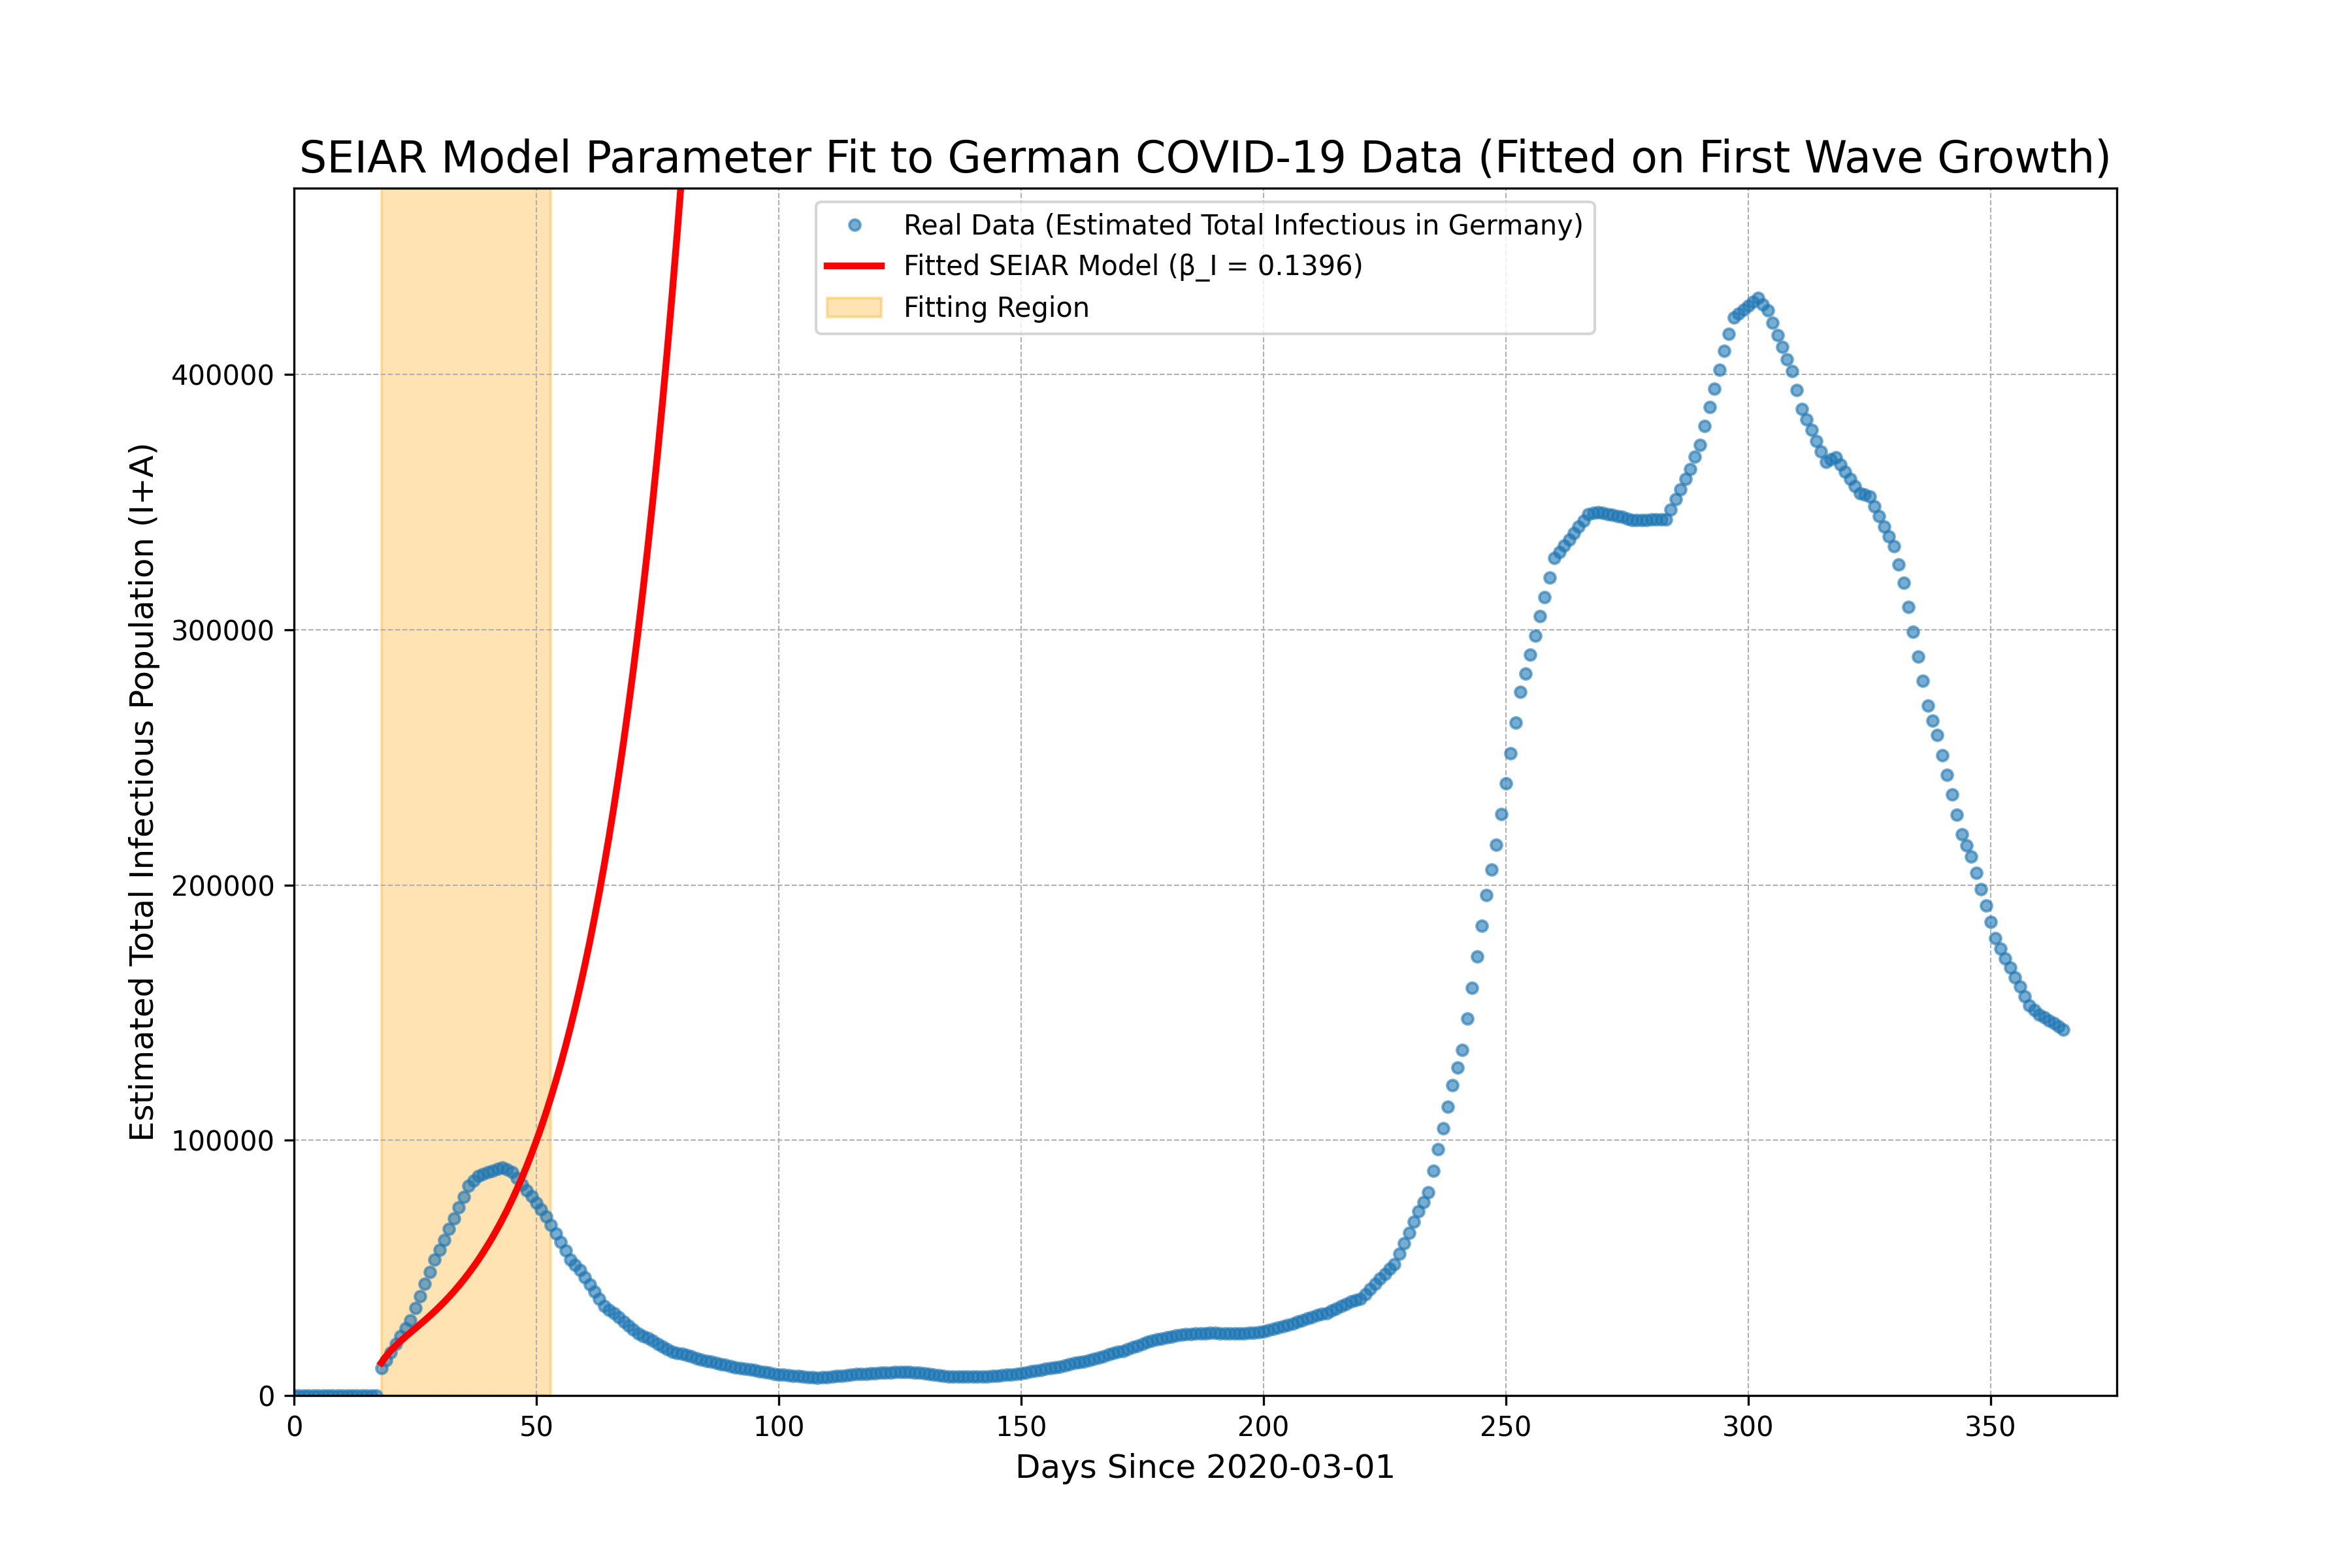
\includegraphics[width=0.8\textwidth]{1/linear_0.png}
    \caption{Fitting on the initial exponential growth phase (days 18-50) leads to an unrealistic projection of uncontrolled growth.}
    \label{fig:linear_0}
\end{figure}

\paragraph{Attempt 3: Piecewise Fitting based on Intervention}
Recognizing that Germany implemented a national lockdown around day 22, we "split" the data at this point and fitted two separate $\beta$ values. The result in Figure \ref{fig:linear_1} is far superior to previous attempts, with the model curve (red line) tracking the data much more closely in both phases. This approach successfully quantifies the effect of the intervention.

\begin{figure}[h!]
    \centering
    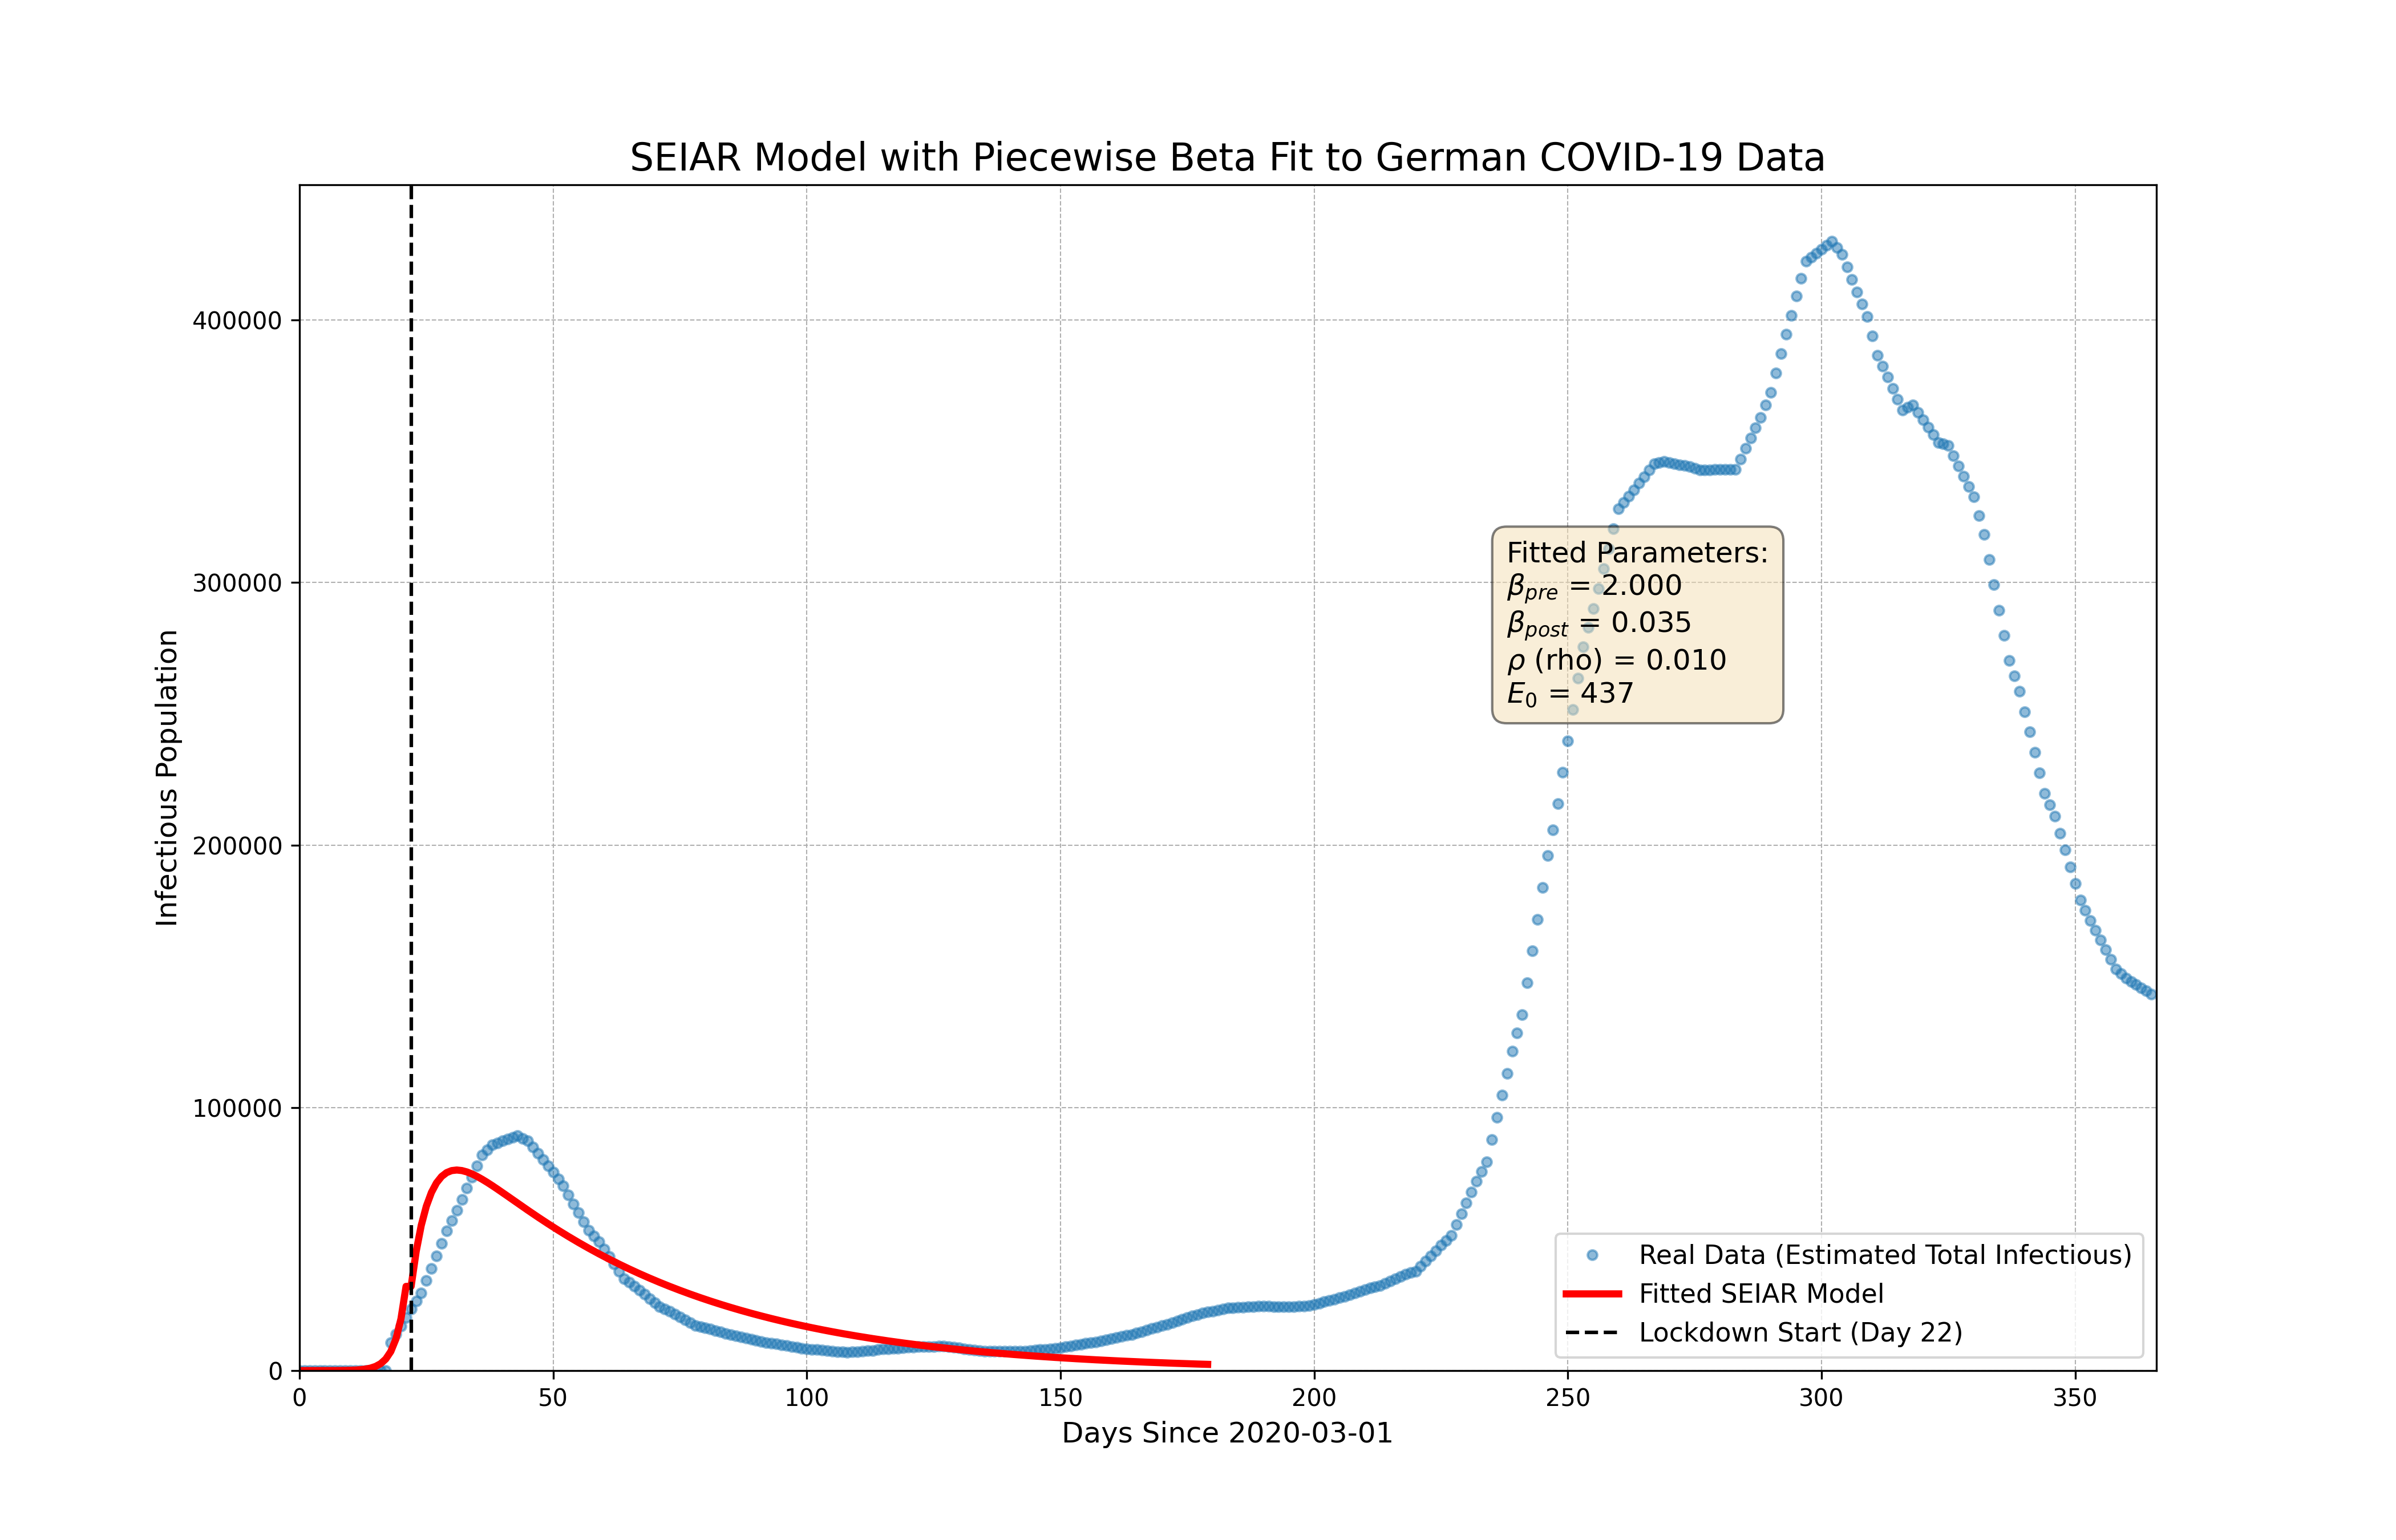
\includegraphics[width=0.8\textwidth]{1/linear_1.png}
    \caption{A two-stage piecewise fit, with the parameter change aligned with the national lockdown, provides a much better description of the first wave.}
    \label{fig:linear_1}
\end{figure}

\paragraph{Final Deterministic Strategy: Multi-Stage Piecewise Fitting}
Building on this success, we extended the concept to a four-stage model across the first 270 days. As shown in Figure \ref{fig:linear_2}, this multi-stage model achieves a very close fit to the complex data dynamics.

\begin{figure}[h!]
    \centering
    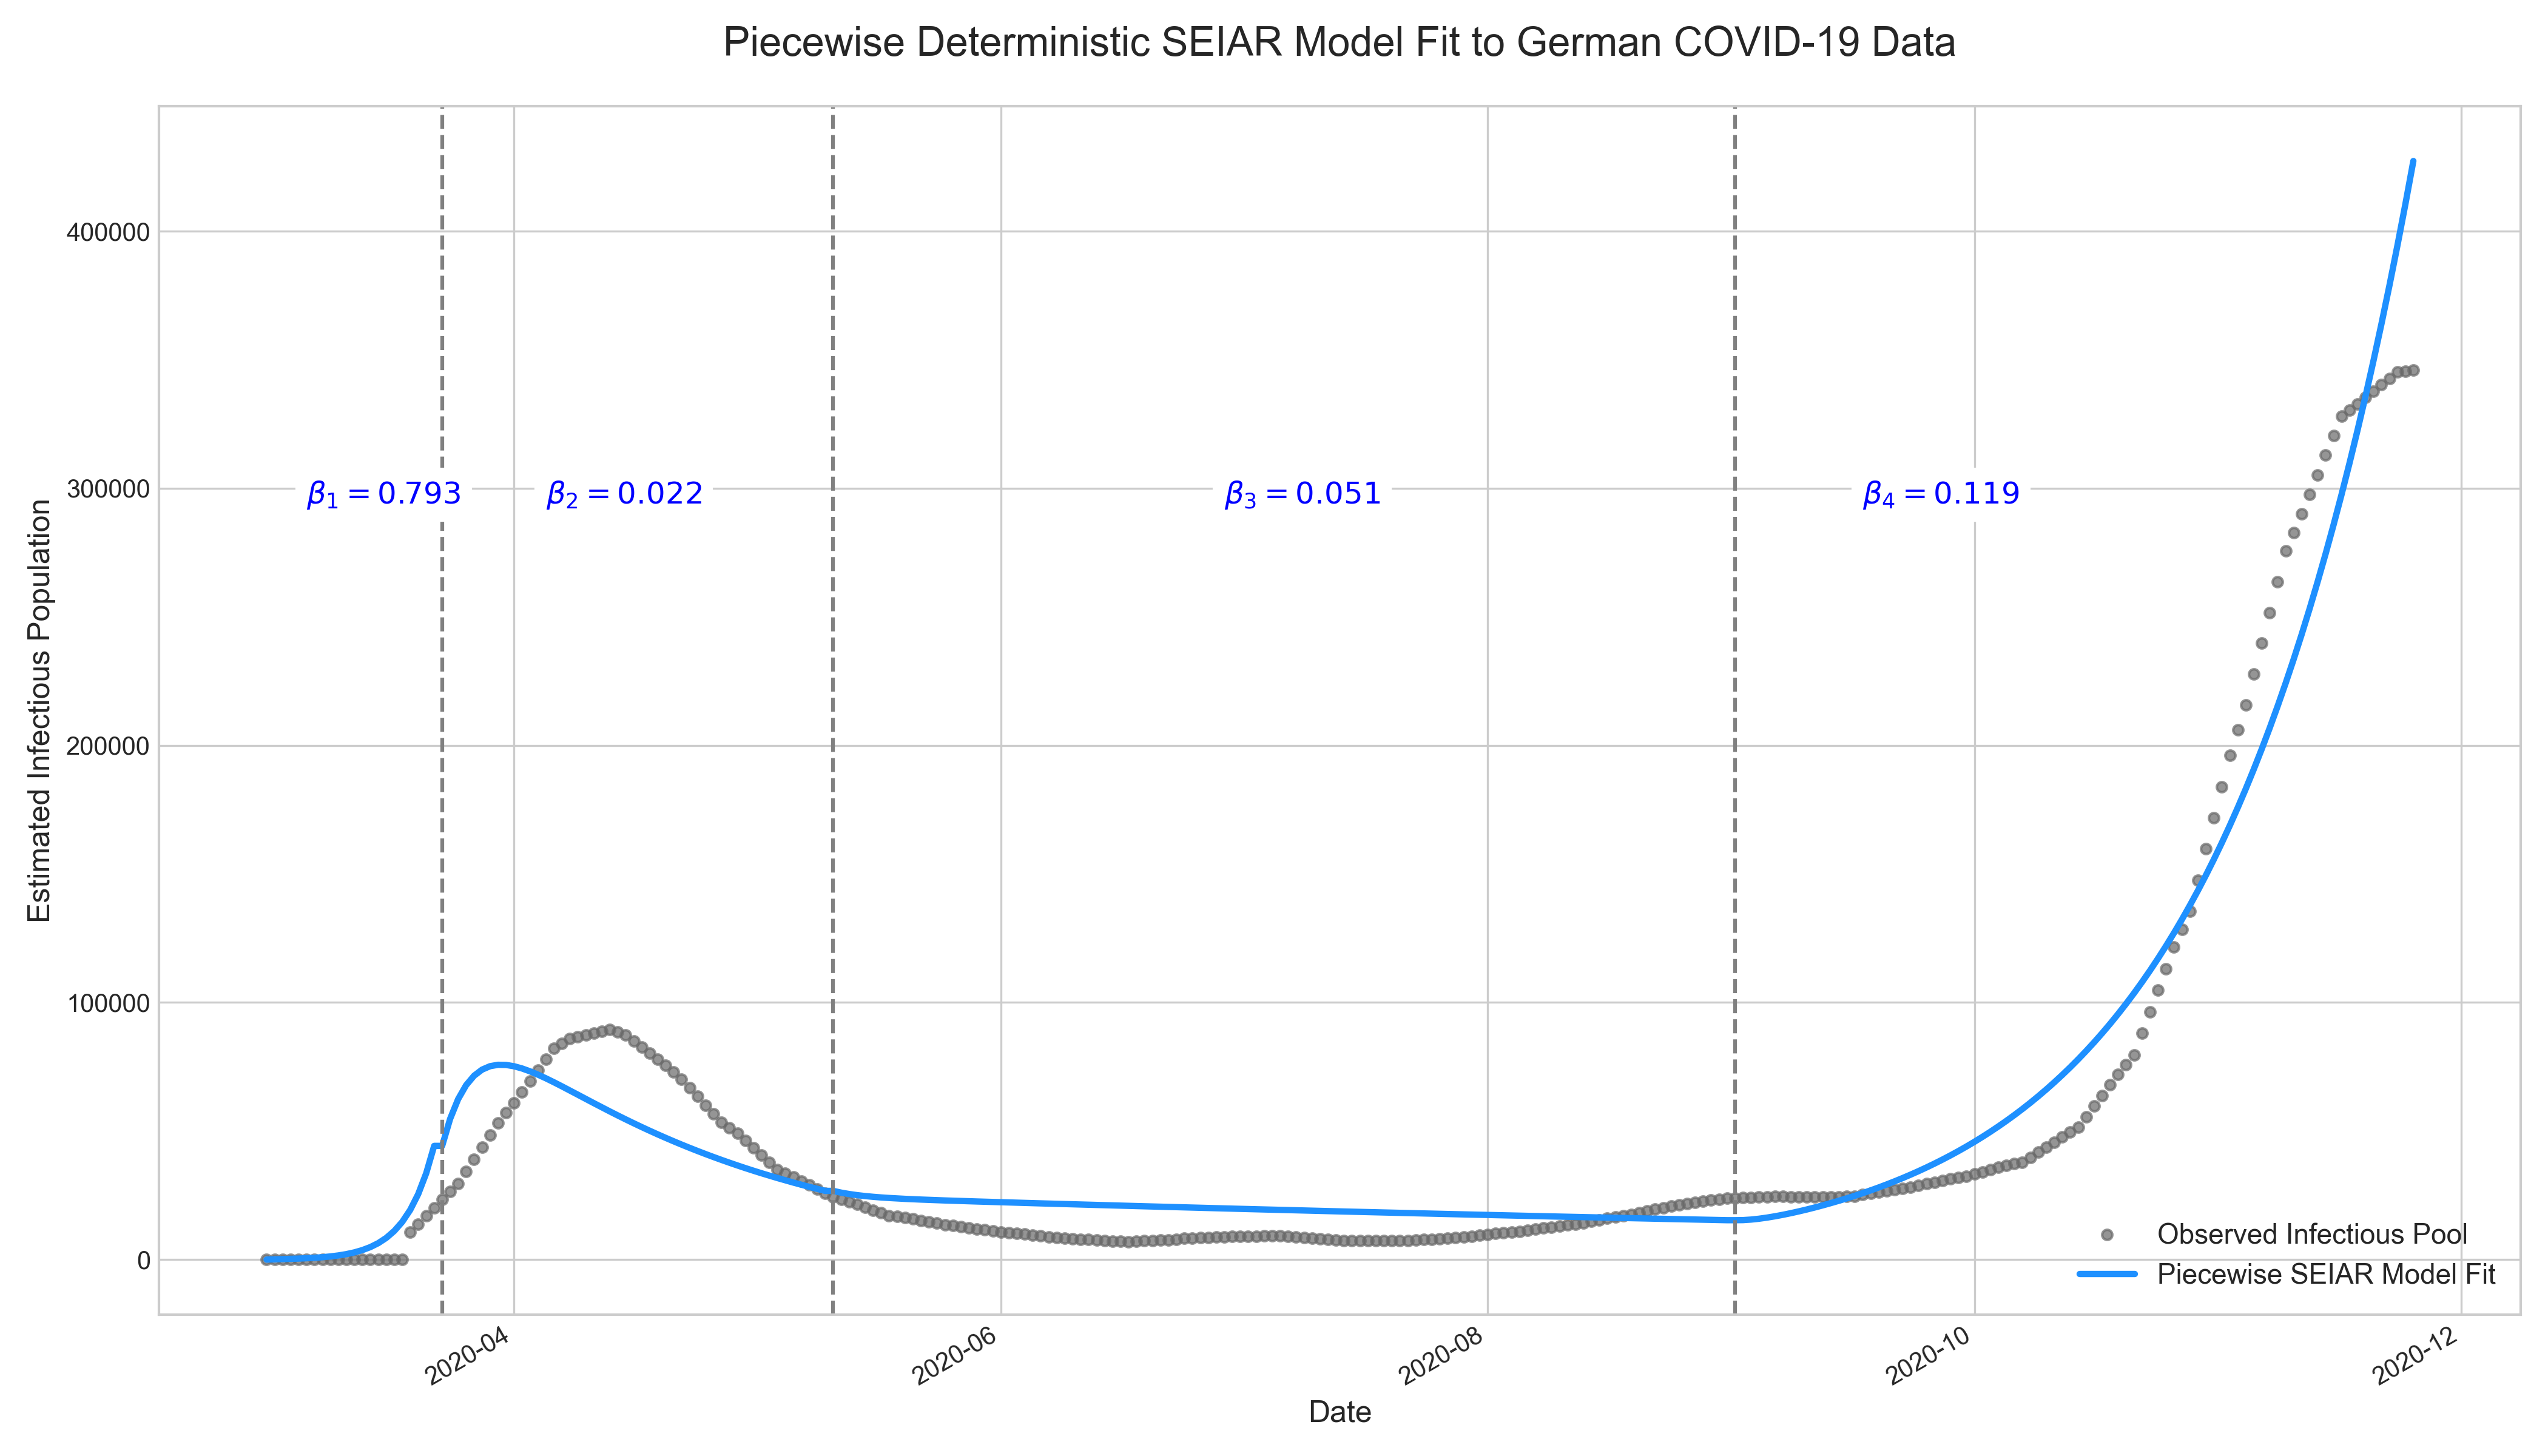
\includegraphics[width=0.8\textwidth]{1/linear_2.png}
    \caption{A four-stage piecewise deterministic model fit over 270 days, demonstrating high fidelity to the observed data.}
    \label{fig:linear_2}
\end{figure}

\subsubsection{Conclusion of Phase 1}
This iterative process led to a clear conclusion: a single, constant $\beta$ parameter is insufficient to model a real-world epidemic. A piecewise parameter model is necessary to capture the dynamic changes in transmission rates. While the least squares method allowed us to quickly validate this strategy, it cannot provide a measure of uncertainty for the estimated parameters. To address this, we advanced to a full Bayesian inference framework in the next phase.

\subsection{Phase 2: Bayesian Inference with Multi-Stage Piecewise Parameters}
To address the limitations of deterministic fitting—namely its inability to model dynamic changes and quantify parameter uncertainty—we advanced to a full Bayesian framework. This approach does not seek a single best-fit solution, but instead aims to infer the complete posterior probability distribution for all unknown parameters, providing a comprehensive understanding of the model's uncertainty.

\subsubsection{Advanced Model Formulation}
The Bayesian model was constructed using the PyMC probabilistic programming library, with the Markov Chain Monte Carlo (MCMC) algorithm as the computational engine for inference. The model design incorporates several key enhancements to better reflect real-world dynamics:
\begin{itemize}
    \item \textbf{Piecewise Parameters ($\beta_t, \rho_t$):} To capture the impact of public health interventions, the time series of the first 270 days was divided into four distinct stages. These stages correspond to different phases of the epidemic in Germany (e.g., initial outbreak, post-lockdown, summer lull, and the beginning of the autumn wave). Each stage was assigned its own independent transmission rate ($\beta_t$) and reporting rate ($\rho_t$), allowing the model to flexibly adapt to the changing transmission environment.
    \item \textbf{Observation Model ($\rho_t$):} We explicitly introduced a reporting rate parameter, $\rho_t$, to account for the discrepancy between the "true" number of infected individuals in the model (I+A) and the "observed" cases in our data. The likelihood function assumes that the observed data is a fraction ($\rho_t$) of the true total, where $\rho_t$ is itself an unknown parameter to be inferred.
    \item \textbf{Informative Priors:} We defined priors for all unknown parameters based on established epidemiological knowledge. A key example is the prior for the initial transmission rate, $\beta_1$. Based on plausible values for the basic reproduction number ($R_0$) during the early COVID-19 pandemic, we set a strong, informative Gamma prior on $\beta_1$ to constrain the MCMC sampler to a realistic parameter space and ensure numerical stability.
    \item \textbf{Likelihood Function:} A Negative Binomial distribution was used for the likelihood. This choice is more robust for epidemic case counts, which often exhibit overdispersion (variance greater than the mean), than a standard Poisson or Normal distribution.
\end{itemize}

\subsubsection{Results and Analysis}
The MCMC simulation successfully converged, producing robust posterior distributions for all unknown parameters. The statistical summary, including the mean, standard deviation, and 94\% highest density interval (credible interval) for each parameter, is presented in Table \ref{tab:mcmc_summary_2}.

\begin{table}[h!]
\centering
\caption{Statistical Summary of Posterior Distributions from MCMC Simulation}
\label{tab:mcmc_summary_2}
\resizebox{\textwidth}{!} & \textbf{hdi\_97\%} & \textbf{mcse\_mean} & \textbf{mcse\_sd} & \textbf{ess\_bulk} & \textbf{ess\_tail} & \textbf{r\_hat} \\
\hline
$\beta_1$ & 1.628 & 0.168 & 1.323 & 1.947 & 0.032 & 0.023 & 29.0 & 74.0 & 1.17 \\
$\beta_2$ & 0.027 & 0.007 & 0.013 & 0.041 & 0.001 & 0.000 & 112.0 & 191.0 & 1.02 \\
$\beta_3$ & 0.057 & 0.002 & 0.053 & 0.061 & 0.000 & 0.000 & 550.0 & 989.0 & 1.00 \\
$\beta_4$ & 0.117 & 0.005 & 0.108 & 0.126 & 0.000 & 0.000 & 1466.0 & 2442.0 & 1.00 \\
$\rho_1$ & 0.122 & 0.037 & 0.057 & 0.193 & 0.004 & 0.003 & 98.0 & 164.0 & 1.03 \\
$\rho_2$ & 0.586 & 0.111 & 0.371 & 0.787 & 0.007 & 0.005 & 238.0 & 310.0 & 1.02 \\
$\rho_3$ & 0.221 & 0.060 & 0.114 & 0.335 & 0.005 & 0.004 & 140.0 & 295.0 & 1.02 \\
$\rho_4$ & 0.285 & 0.089 & 0.136 & 0.464 & 0.007 & 0.005 & 158.0 & 252.0 & 1.02 \\
$E_0$ & 32.476 & 23.210 & 5.499 & 76.054 & 3.938 & 2.808 & 31.0 & 60.0 & 1.09 \\
$\text{noise}_{\alpha}$ & 2.322 & 0.255 & 1.860 & 2.804 & 0.025 & 0.018 & 107.0 & 516.0 & 1.02 \\
\hline
\end{tabular}
}
\end{table}

The final model fit is shown in Figure \ref{fig:bayesian_fit_2}. The model, with its piecewise parameters, successfully captures the complex dynamics of the German epidemic over the 270-day period. This includes the initial rise, the turning point corresponding to the lockdown, the subsequent decline, and the resurgence of cases in the autumn.

\begin{figure}[h!]
    \centering
    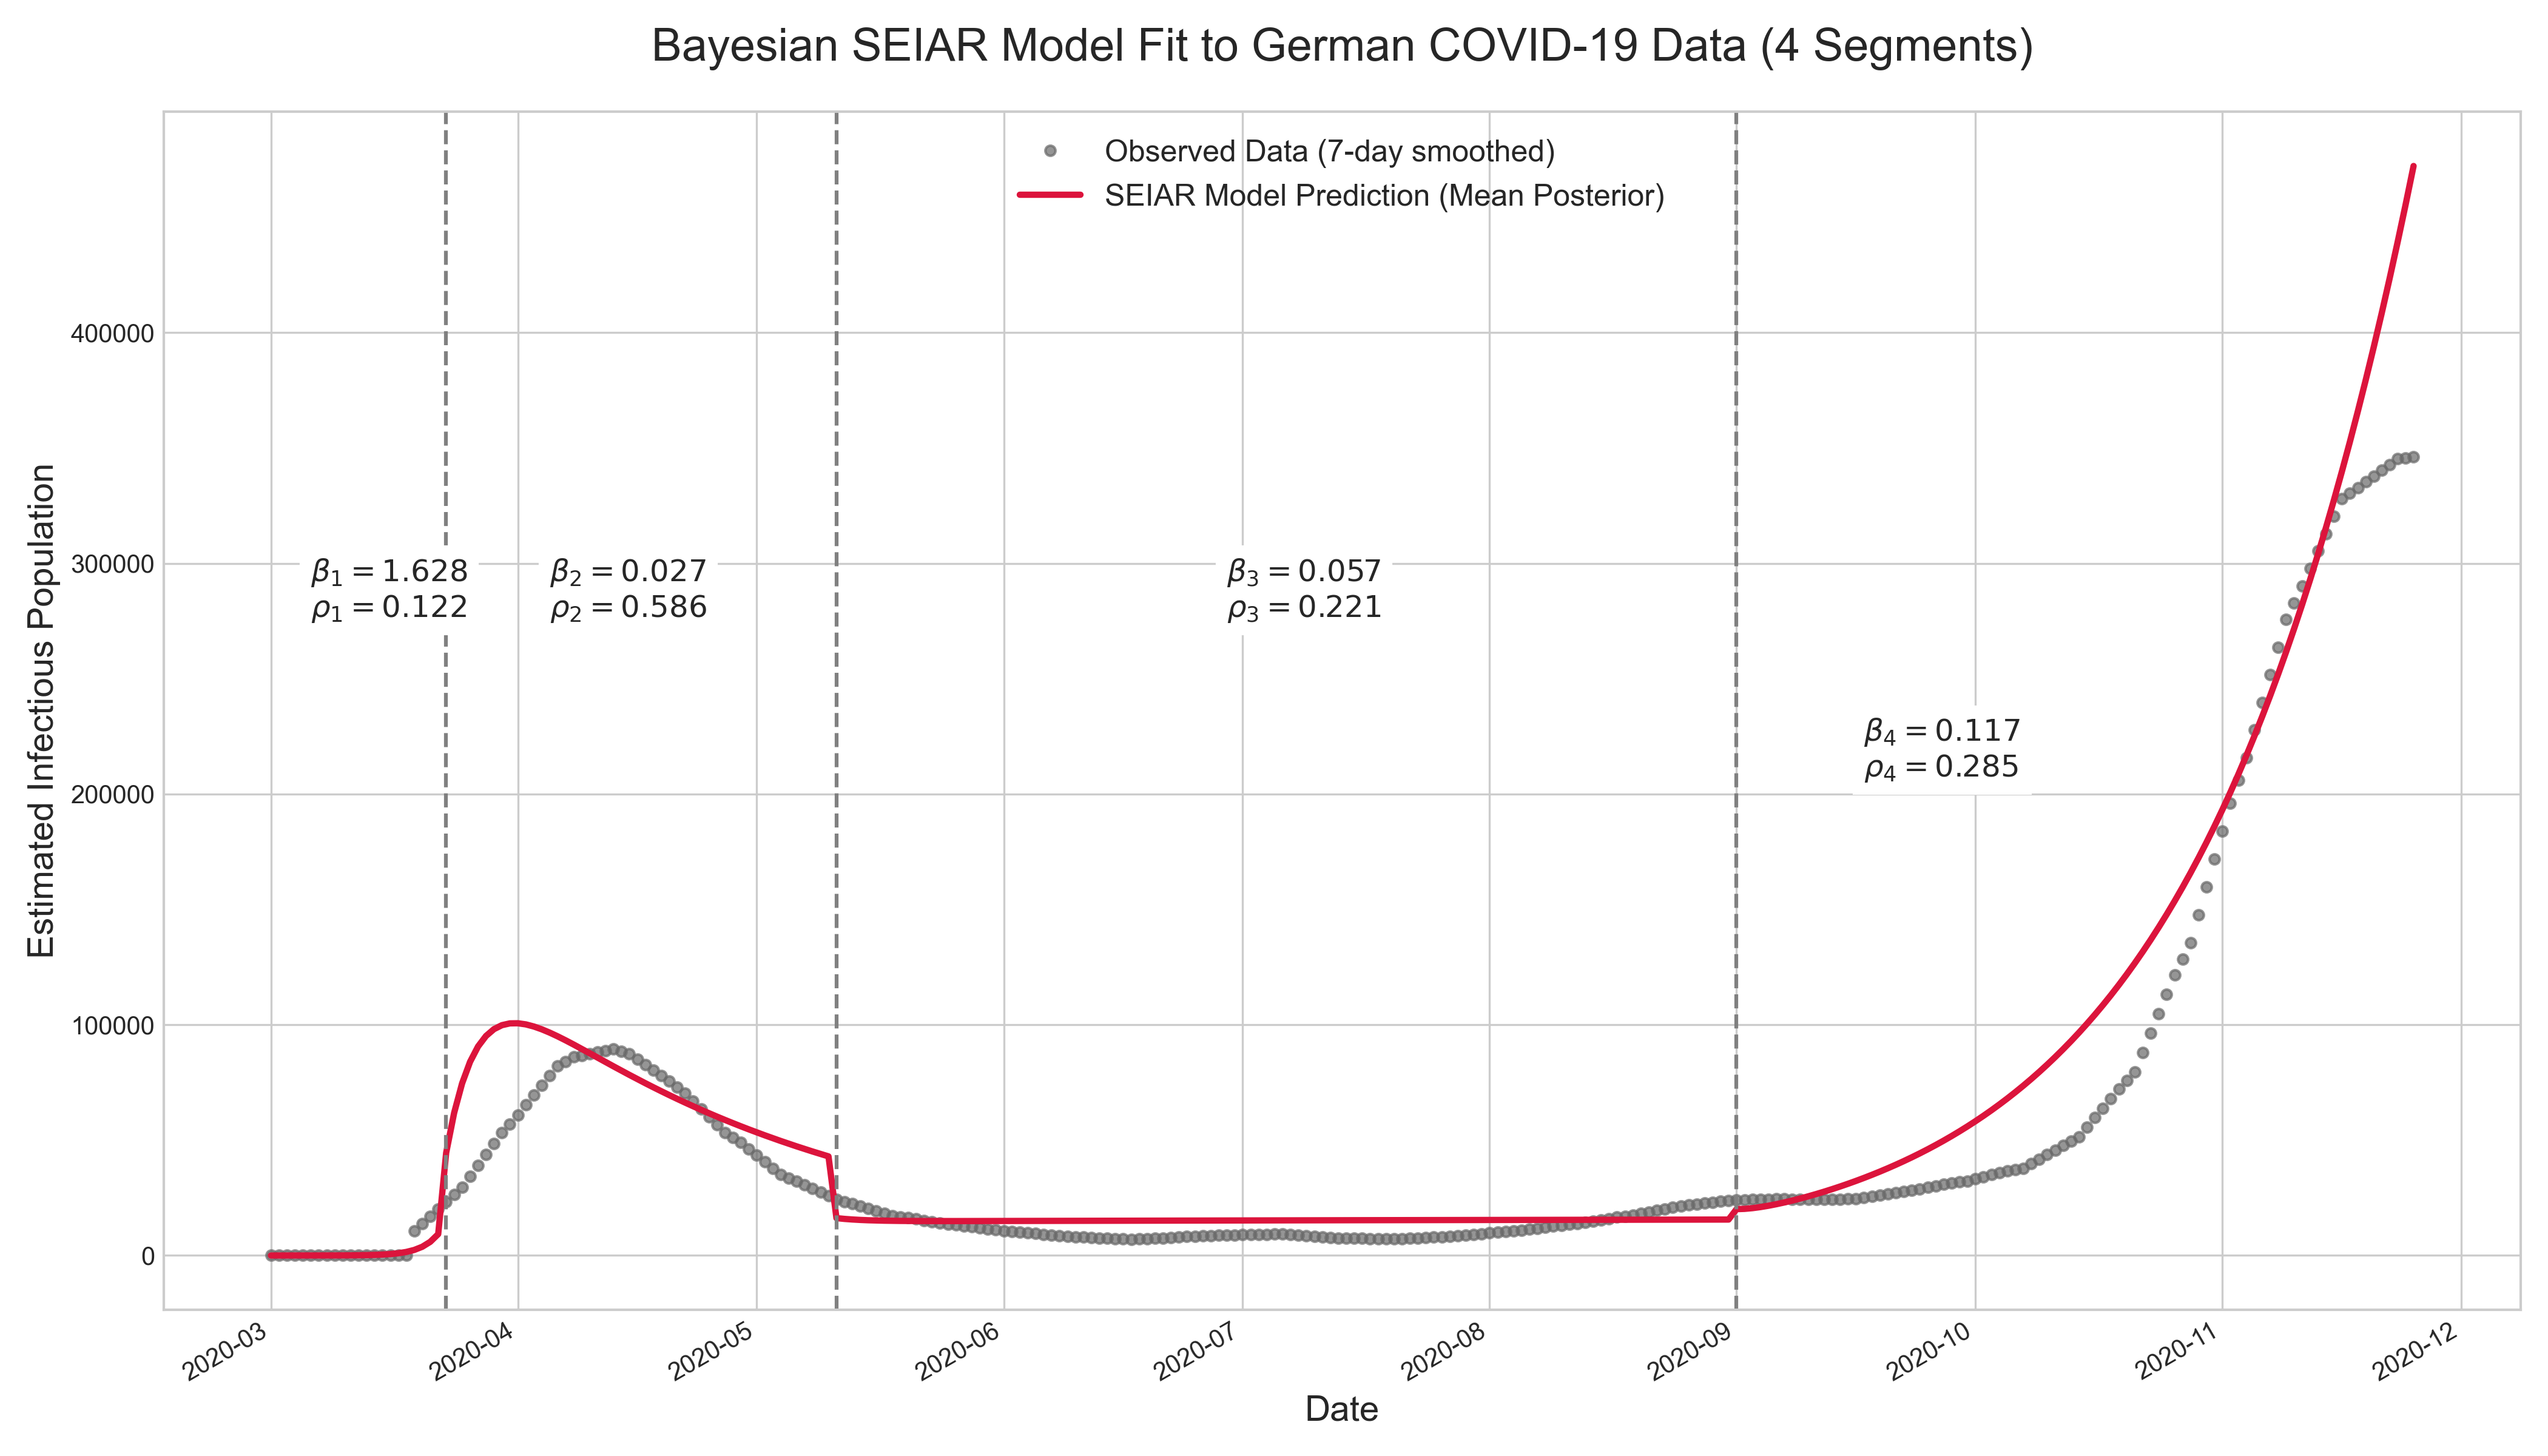
\includegraphics[width=0.9\textwidth]{1/bayesian_fit_to_data.png}
    \caption{Final Bayesian model fit against observed German COVID-19 data. The shaded region represents the 94\% highest posterior density interval of the model's prediction.}
    \label{fig:bayesian_fit_2}
\end{figure}

The posterior distributions (Figure \ref{fig:posterior_plots_2}) provide a visual representation of the estimated value and uncertainty for each parameter. By analyzing these results, we can quantitatively interpret the epidemic's evolution. For instance, the model estimates a significant drop in the transmission rate $\beta_t$ after the lockdown was implemented around day 22, providing clear evidence for the effectiveness of the intervention.

\begin{figure}[h!]
    \centering
    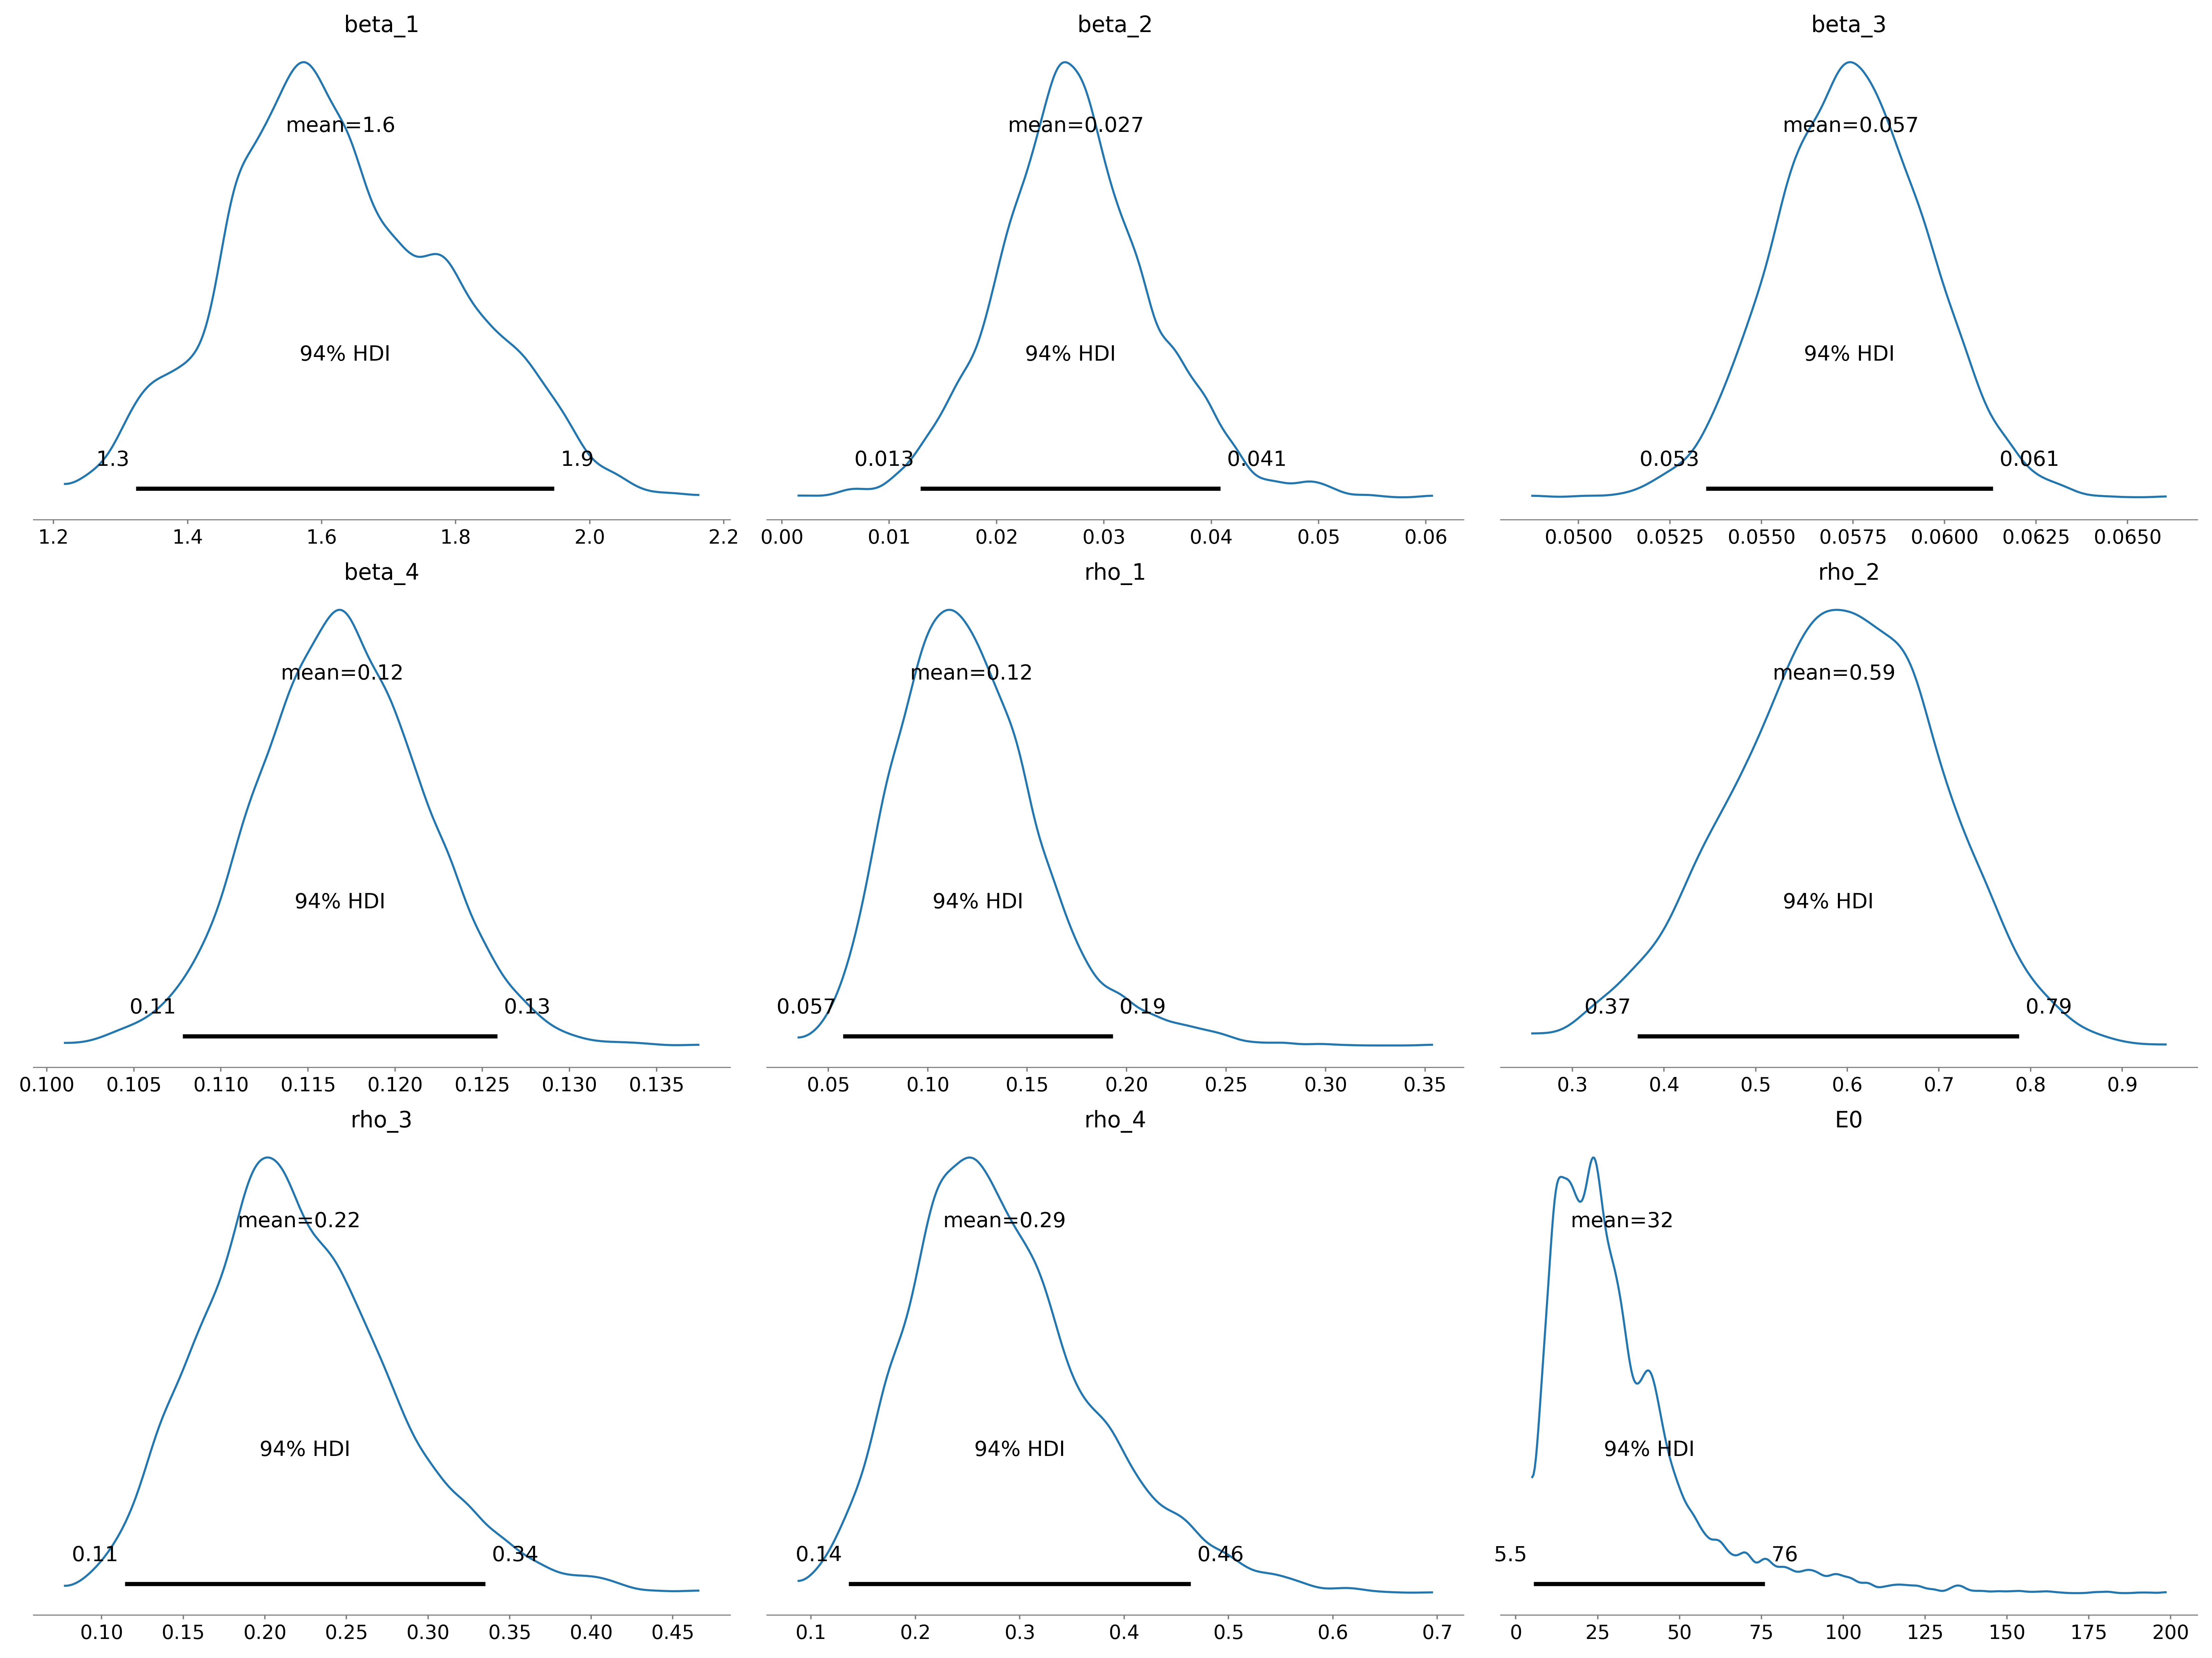
\includegraphics[width=\textwidth]{1/bayesian_posterior_plots.png}
    \caption{Posterior distributions for the piecewise transmission rates ($\beta_t$), reporting rates ($\rho_t$), initial exposed population ($E_0$), and observation noise.}
    \label{fig:posterior_plots_2}
\end{figure}

\subsection{Simulation and Scenario Analysis}
With a fully calibrated and validated dynamic model from the Bayesian inference phase, we can now utilize it as a predictive tool to conduct scenario analysis. This step addresses the requirement in the project outline to compare simulations under different conditions and demonstrates the model's practical utility for informing public health policy.

\subsubsection{Methodology}
We investigate the example question posed by the project brief: "How does a 20\% reduction in contact rate affect the peak number of infections?". To answer this, we simulate two distinct scenarios:
\begin{itemize}
    \item \textbf{Baseline Scenario:} This scenario represents the "natural" course of an unmitigated outbreak. We use the posterior mean of the transmission rate estimated for the first, pre-lockdown phase of the epidemic ($\beta_1$) as our baseline parameter.
    \item \textbf{Intervention Scenario:} This scenario models the effect of a public health intervention that successfully reduces contact rates by 20\%. In our model, this is equivalent to reducing the transmission rate by 20\%. The new parameter is thus set to $\beta_{\text{intervention}} = 0.8 \times \beta_1$.
\end{itemize}
Both simulations were initiated with the same starting conditions (e.g., the posterior mean of $E_0$ from our Bayesian analysis) and run for a 365-day period to observe the full development of the epidemic wave.

\subsubsection{Results and Discussion}
The outcomes of the two simulations are visualized in Figure \ref{fig:scenario_sim}. The plot clearly illustrates the powerful impact of reducing the transmission rate.

\begin{figure}[h!]
    \centering
    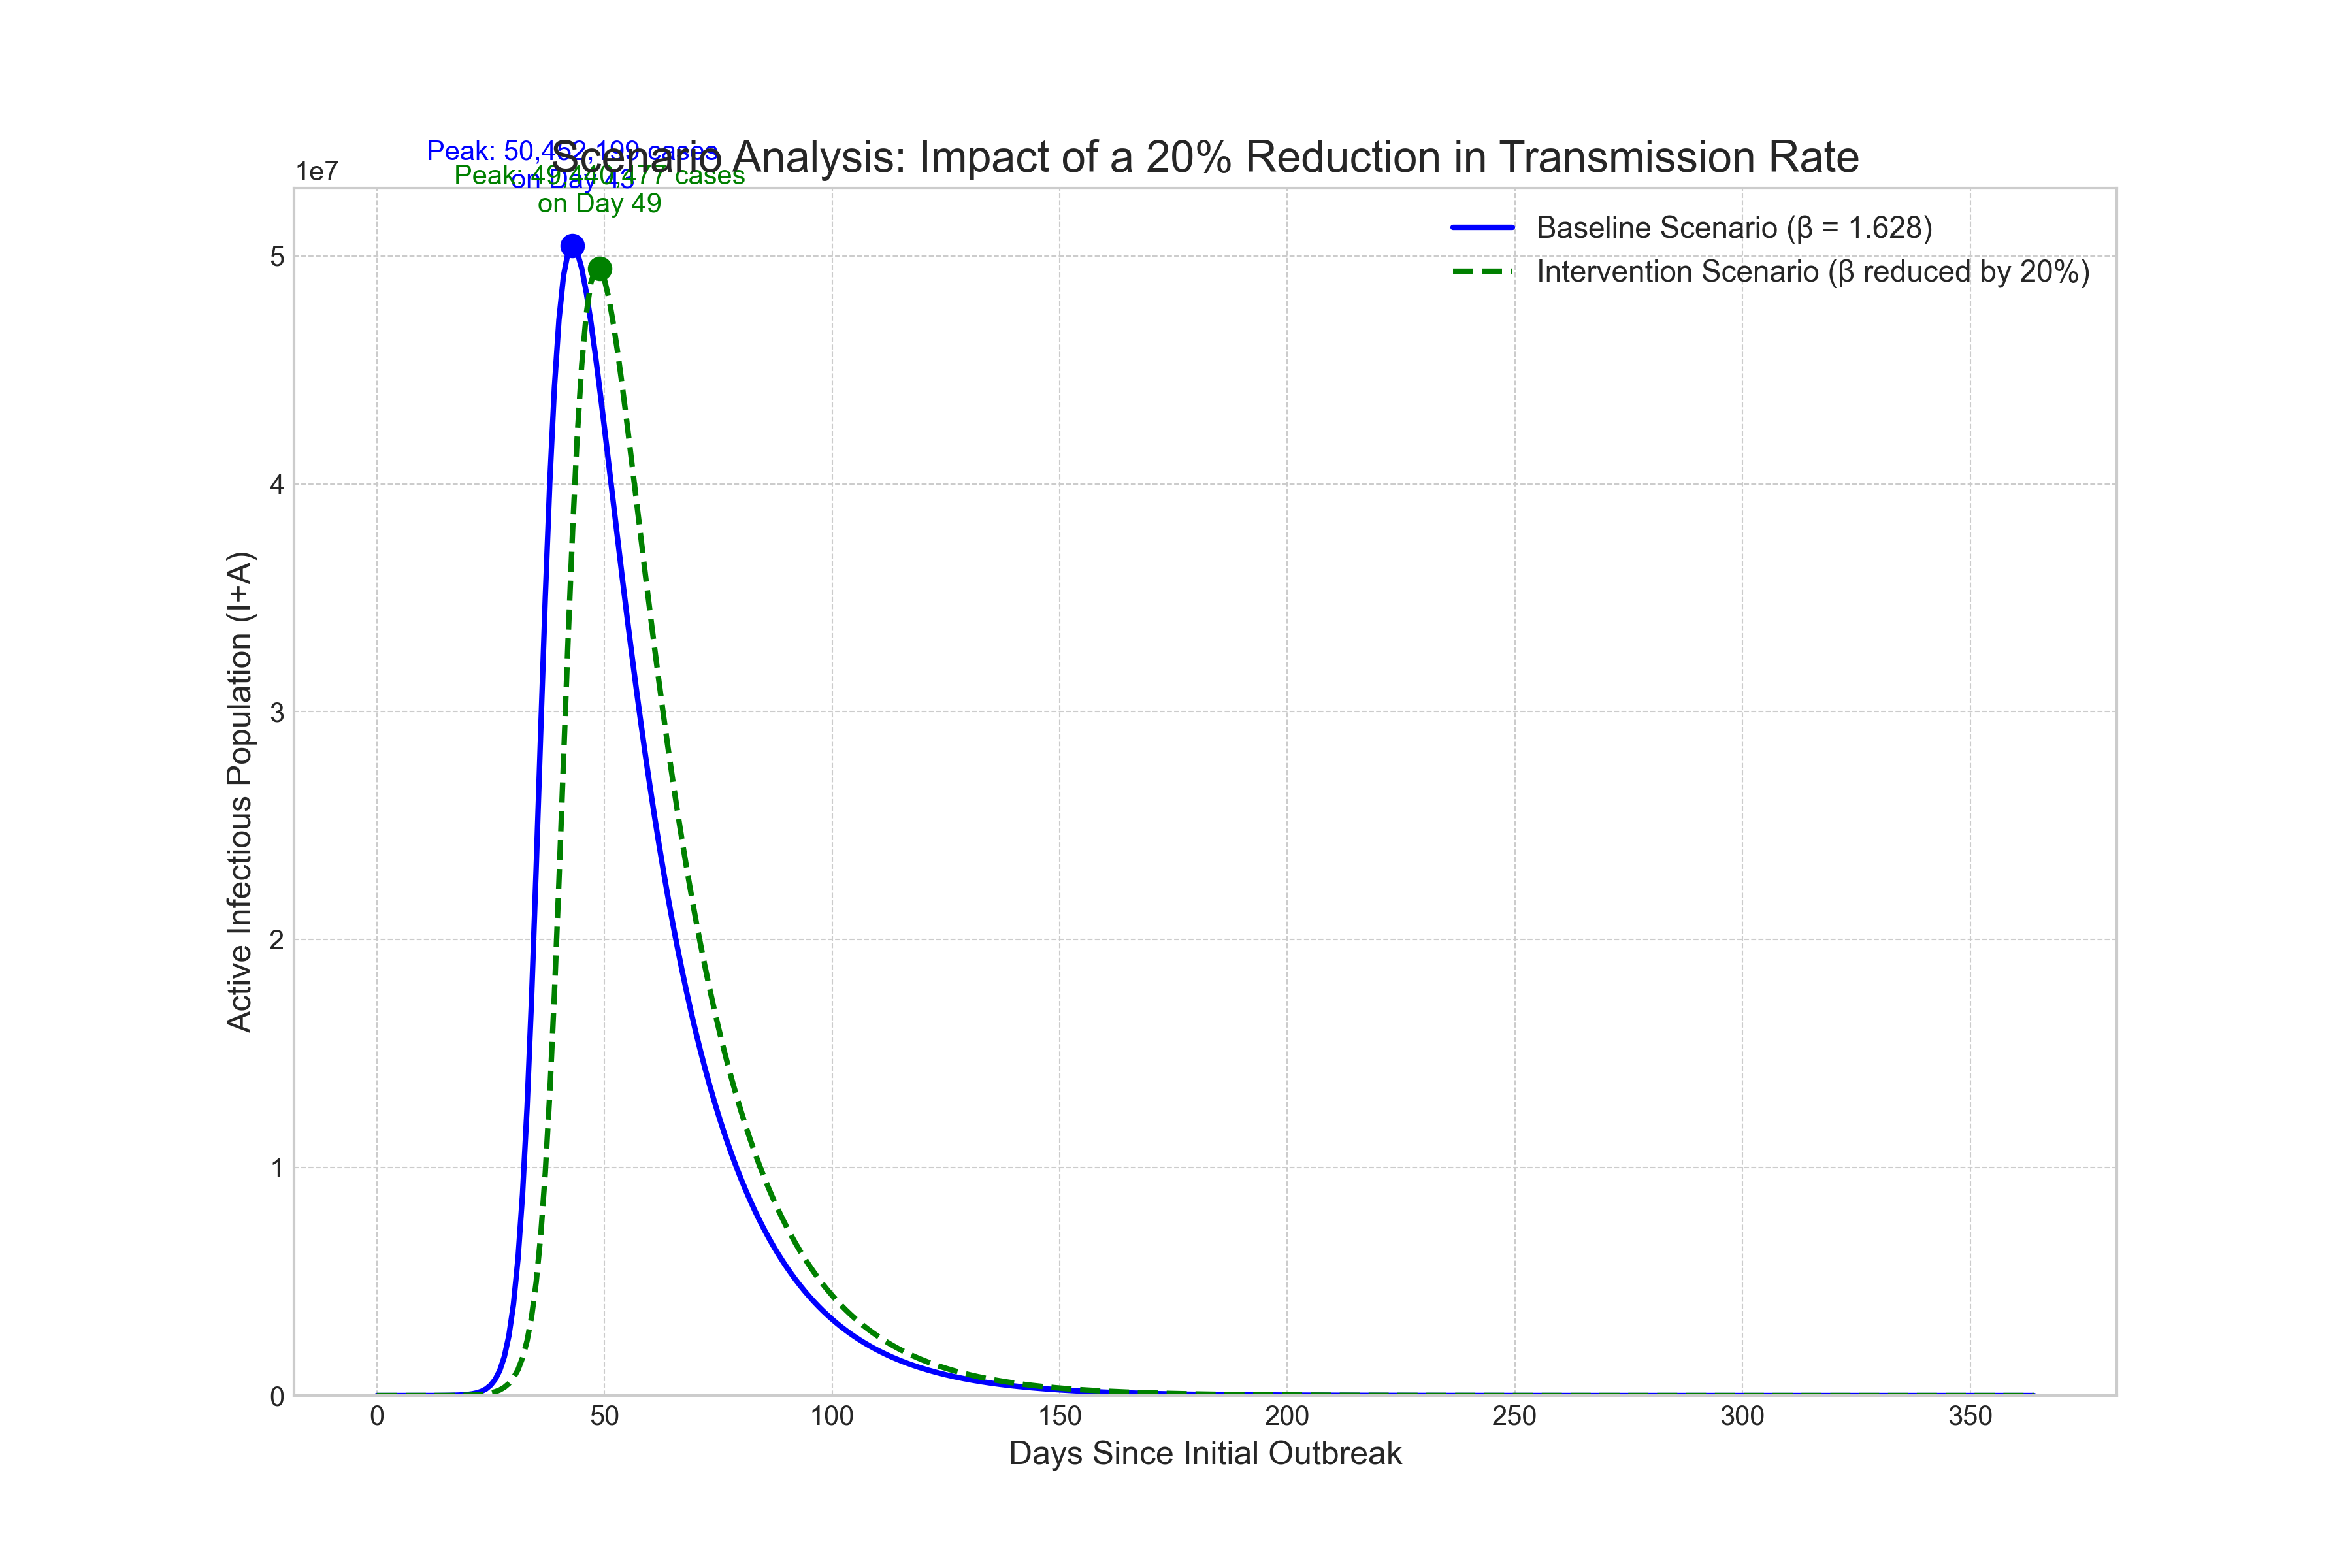
\includegraphics[width=0.8\textwidth]{1/scenario_simulation.png}
    \caption{Comparison of epidemic trajectories under a baseline scenario versus an intervention scenario with a 20\% reduction in the transmission rate.}
    \label{fig:scenario_sim}
\end{figure}

In the baseline scenario, the epidemic grows rapidly, leading to a significant peak in the number of active infectious individuals. In contrast, the intervention scenario shows a dramatically different trajectory. The analysis of the simulation results reveals that:
\begin{itemize}
    \item The 20\% reduction in the transmission rate successfully "flattens the curve."
    \item Specifically, while the relative reduction in the peak number of infections is 2.0\%, this corresponds to an absolute reduction of over one million peak infections (from approx. 50.5 million to 49.4 million). This represents a massive decrease in the instantaneous burden on the healthcare system.
    \item Furthermore, the intervention delays the peak of the epidemic from day 43 to day 49. This delay of 6 days provides a valuable window for policy response and resource allocation.
\end{itemize}
This quantitative analysis demonstrates the profound effectiveness of public health measures aimed at reducing contact rates. A modest 20\% reduction can drastically lower the peak burden on the healthcare system and provide valuable extra time for preparation and response. This underscores the critical importance of non-pharmaceutical interventions like social distancing in managing an epidemic outbreak.

\section{Part 4: Critical Analysis and Discussion}
Having successfully constructed and calibrated an SEIAR model capable of describing the dynamics of the COVID-19 epidemic, this final section provides a critical analysis of the model's limitations, potential avenues for improvement, and its implications for real-world policy decisions, as required by the project outline.

\subsection{Limitations of the Model}
While our final Bayesian model achieved a strong fit to the observed data, it is built upon a series of simplifying assumptions that constitute its primary limitations.

\paragraph{Assumption of Homogeneous Mixing} The SEIAR model assumes that individuals within each compartment are homogeneous and mix randomly. This ignores critical population structures, such as age demographics and social contact networks. In reality, the contact patterns of school-aged children are vastly different from those of office workers or retirees, which significantly affects disease transmission pathways. This limitation may be reflected in our Bayesian inference results. For instance, the posterior distribution for the initial transmission rate, $\beta_1$, has a relatively wide 94\% credible interval (Table \ref{tab:mcmc_summary_2}). This uncertainty could partially stem from the model's inability to capture the heterogeneous transmission dynamics present in the real population during the initial, uncontrolled phase of the outbreak.

\paragraph{Lack of Spatial Dynamics} Our model is non-spatial, treating the entire country as a single, well-mixed population. It does not capture the geographical heterogeneity of the outbreak, where urban centers may act as epicenters while rural areas experience different dynamics.

\paragraph{Assumption of Permanent Immunity} The model assumes that individuals in the Recovered (R) compartment gain permanent immunity. For a disease like COVID-19, it is now understood that immunity can wane over time and reinfection is possible. Our model does not include a pathway from the R to the S compartment and is therefore not suited for modeling long-term, multi-wave dynamics where waning immunity is a factor.

\paragraph{Limitation of Piecewise-Constant Parameters} A more subtle limitation lies in our use of piecewise-constant parameters. While modeling $\beta_t$ and $\rho_t$ in distinct stages is a significant improvement over a single constant parameter, it still assumes these rates are fixed within each stage. In reality, factors like policy implementation and public behavioral changes are gradual. Therefore, a truly realistic model might represent these parameters as continuous functions, $\beta(t)$ and $\rho(t)$, that change smoothly over time. Our piecewise model can be seen as a first-order approximation of this continuous reality, capturing the major turning points but not the subtle variations within each phase.

\subsection{Methodological Reflections and Future Improvements}
The modeling process itself provided valuable lessons, particularly regarding the methodology of parameter inference.

\paragraph{Insights from MCMC Debugging} During the development of the Bayesian model, we encountered and resolved a classic "prior-likelihood conflict," which initially prevented the MCMC simulation from converging. This challenge highlighted the critical importance of integrating domain knowledge into the modeling process. By using established epidemiological knowledge about the plausible range of $R_0$ to construct an informative prior for the initial transmission rate ($\beta_1$), we successfully resolved the model's identifiability issues and achieved convergence. This debugging journey itself is a testament to the power of combining data, a flexible model structure, and prior knowledge in complex systems modeling.

\paragraph{Potential Model Improvements} Corresponding to the limitations identified above, several avenues exist for future improvement:
\begin{itemize}
    \item \textbf{More Realistic Parameter Dynamics:} Higher-order methods, such as splines or Gaussian Processes, could be used to model $\beta(t)$ as a continuous function.
    \item \textbf{Age-Structured Model:} The population could be stratified into different age groups, with an interaction matrix defining the contact rates between them.
    \item \textbf{Spatial Metapopulation Model:} The model could be extended to a spatial framework, dividing Germany into geographic regions (e.g., states) with migration and commuting flows modeled between them.
    \item \textbf{Immunity Waning:} An SEIRS model could be implemented, allowing individuals to return from the Recovered to the Susceptible class at a specified rate.
    \item \textbf{Incorporating Vaccination:} As a key public health intervention, vaccination could be added to the model. This would typically involve adding a new compartment, V (Vaccinated), and a flow from S to V at a certain rate $\alpha(t)$, representing the vaccination campaign's rollout. This extension would be crucial for modeling the pandemic's trajectory in 2021 and beyond and for evaluating the population-level impact of different vaccination strategies.
\end{itemize}

\subsection{Findings and Implications for Real-World Policy}
Despite its limitations, our model provides several valuable insights for public health decision-making.

\paragraph{Quantifying the Effectiveness of Interventions} Our piecewise Bayesian model clearly estimated a significant, quantifiable drop in the transmission rate $\beta_t$ following the implementation of lockdown measures in Germany. This provides strong, data-driven evidence supporting the utility of non-pharmaceutical interventions (NPIs) like social distancing in controlling an epidemic.

\paragraph{Highlighting the Role of Asymptomatic Transmission} By explicitly including an asymptomatic compartment (A), our model quantifies the substantial contribution of "silent spreaders" to the epidemic's progression. This finding underscores the critical importance of public health strategies that are not solely reliant on symptom-based case detection, such as mass testing, contact tracing, and the promotion of universal mask-wearing.

\paragraph{Assessing the Impact of Observational Bias} Our inference of a time-varying reporting rate ($\rho_t$) suggests that the number of officially reported cases may represent only a fraction of the true number of infections. This insight is crucial for policymakers, as it implies that the true scale of an outbreak might be significantly underestimated, requiring more proactive and widespread resource allocation for healthcare systems.

\paragraph{Predictive Value of Scenario Analysis} The scenario analysis conducted in Section 3.3 serves as a powerful decision-support tool. It quantifies how a specific measure—such as a "20\% reduction in contact rate"—can effectively "flatten the curve" and delay the epidemic's peak. This provides a scientific basis for weighing the costs and benefits of different intervention strategies during the early stages of a pandemic.


\section{Conclusion}
This project has successfully navigated the complete lifecycle of epidemiological modeling, from foundational theory to data-driven inference and policy-relevant simulation. By systematically building upon the classic SIR model, we developed a sophisticated, multi-stage SEIAR model that accurately captured the complex dynamics of the COVID-19 outbreak in Germany.

The key findings of this report are threefold. First, we demonstrated that simple models with constant parameters are insufficient to describe a real-world epidemic influenced by public health interventions. Our iterative fitting process showed that only a model with time-varying parameters could adequately match the observed data, successfully quantifying the significant reduction in the transmission rate ($\beta_t$) following lockdown measures.

Second, our Bayesian MCMC analysis provided a robust framework for not only estimating parameters but also for quantifying their uncertainty. By explicitly modeling the reporting rate ($\rho_t$), we highlighted the critical discrepancy between reported cases and the true underlying number of infections. This insight, combined with the model's ability to account for asymptomatic transmission, underscores the importance of public health strategies that are not solely reliant on symptom-based surveillance.

Finally, the scenario analysis conducted in Part 3 showcased the practical utility of our calibrated model as a decision-support tool. It quantitatively confirmed that even moderate reductions in the transmission rate can substantially flatten the epidemic curve and delay its peak, providing strong evidence for the effectiveness of non-pharmaceutical interventions.

While our final model represents a significant advancement over simpler frameworks, we acknowledge its limitations, including the assumptions of homogeneous mixing and the absence of spatial dynamics and waning immunity. Future work could address these by developing age-structured or spatial meta-population models. Nevertheless, this project successfully demonstrates how a rigorous, iterative modeling process—combining mathematical theory, statistical inference, and domain knowledge—can yield powerful insights into the dynamics of infectious diseases and their control.

\newpage
\section*{Acknowledgements}
I would like to acknowledge the assistance of Google's Gemini, an AI language model, which was utilized as a valuable tool throughout this project. Its contributions included explaining complex mathematical concepts, debugging code, and assisting in the refinement of the report's text. All final analyses, strategic decisions, and the scientific interpretation of the results are my own work.

% --- 参考文献 (References) ---
\begin{thebibliography}{9}

    % 这是您已有的参考文献,我们保留
    \bibitem{Kermack1927}
    W. O. Kermack and A. G. McKendrick, 
    "A Contribution to the Mathematical Theory of epidemics,"
    \textit{Proceedings of the Royal Society A}, vol. 115, no. 772, pp. 700-721, 1927.

    \bibitem{Chen2014_Book} % Renamed key to avoid conflict
    D. Chen, B. Moulin, and J. Wu, Eds.,
    \textit{Analyzing and Modeling Spatial and Temporal Dynamics of Infectious Diseases}.
    John Wiley \& Sons, Inc., 2014.
    
    % --- 以下是我们为无症状模型新增的核心参考文献 ---

    \bibitem{Byambasuren2020}
    O. Byambasuren, M. Cardona, K. Bell, J. Clark, M.-L. McLaws, and P. Glasziou,
    "Estimating the extent of asymptomatic COVID-19 and its potential for community transmission: Systematic review and meta-analysis,"
    \textit{Official Journal of the Association of Medical Microbiology and Infectious Disease Canada}, vol. 5, no. 4, pp. 224-234, 2020.

    \bibitem{Wang2022}
    Y. Wang, K. Zheng, W. Gao, J. Lv, C. Yu, L. Wang, Z. Wang, B. Wang, C. Liao, and L. Li,
    "Asymptomatic and pre-symptomatic infection in Coronavirus Disease 2019 pandemic,"
    \textit{Medical Reviews}, vol. 2, no. 1, pp. 66-88, 2022.

    \bibitem{Wong2020}
    J. Wong, A. B. Z. Abdul Aziz, L. Chaw, A. Mahamud, M. M. Griffith, Y.-R. Lo, and L. Naing,
    "High proportion of asymptomatic and presymptomatic COVID-19 infections in air passengers to Brunei,"
    \textit{Journal of Travel Medicine}, vol. 27, no. 5, p. taaa066, 2020.

    \bibitem{Chen2021}
    X. Chen, Z. Huang, J. Wang, M. C.-S. Wong, K. C. Chong, S. Zhao, D. He, and J. Li,
    "Ratio of asymptomatic COVID-19 cases among ascertained SARS-CoV-2 infections in different regions and population groups in 2020: a systematic review and meta-analysis,"
    \textit{BMJ Open}, vol. 11, no. 12, p. e049752, 2021.

    \bibitem{vandenDriessche2002}
    P. van den Driessche and J. Watmough,
    "Reproduction numbers and sub-threshold endemic equilibria for compartmental models of disease transmission,"
    \textit{Mathematical Biosciences}, vol. 180, no. 1-2, pp. 29-48, 2002.
    
\end{thebibliography}

\clearpage
\appendix
\section{MCMC Convergence Diagnostics}
\begin{figure}[H]
    \centering
    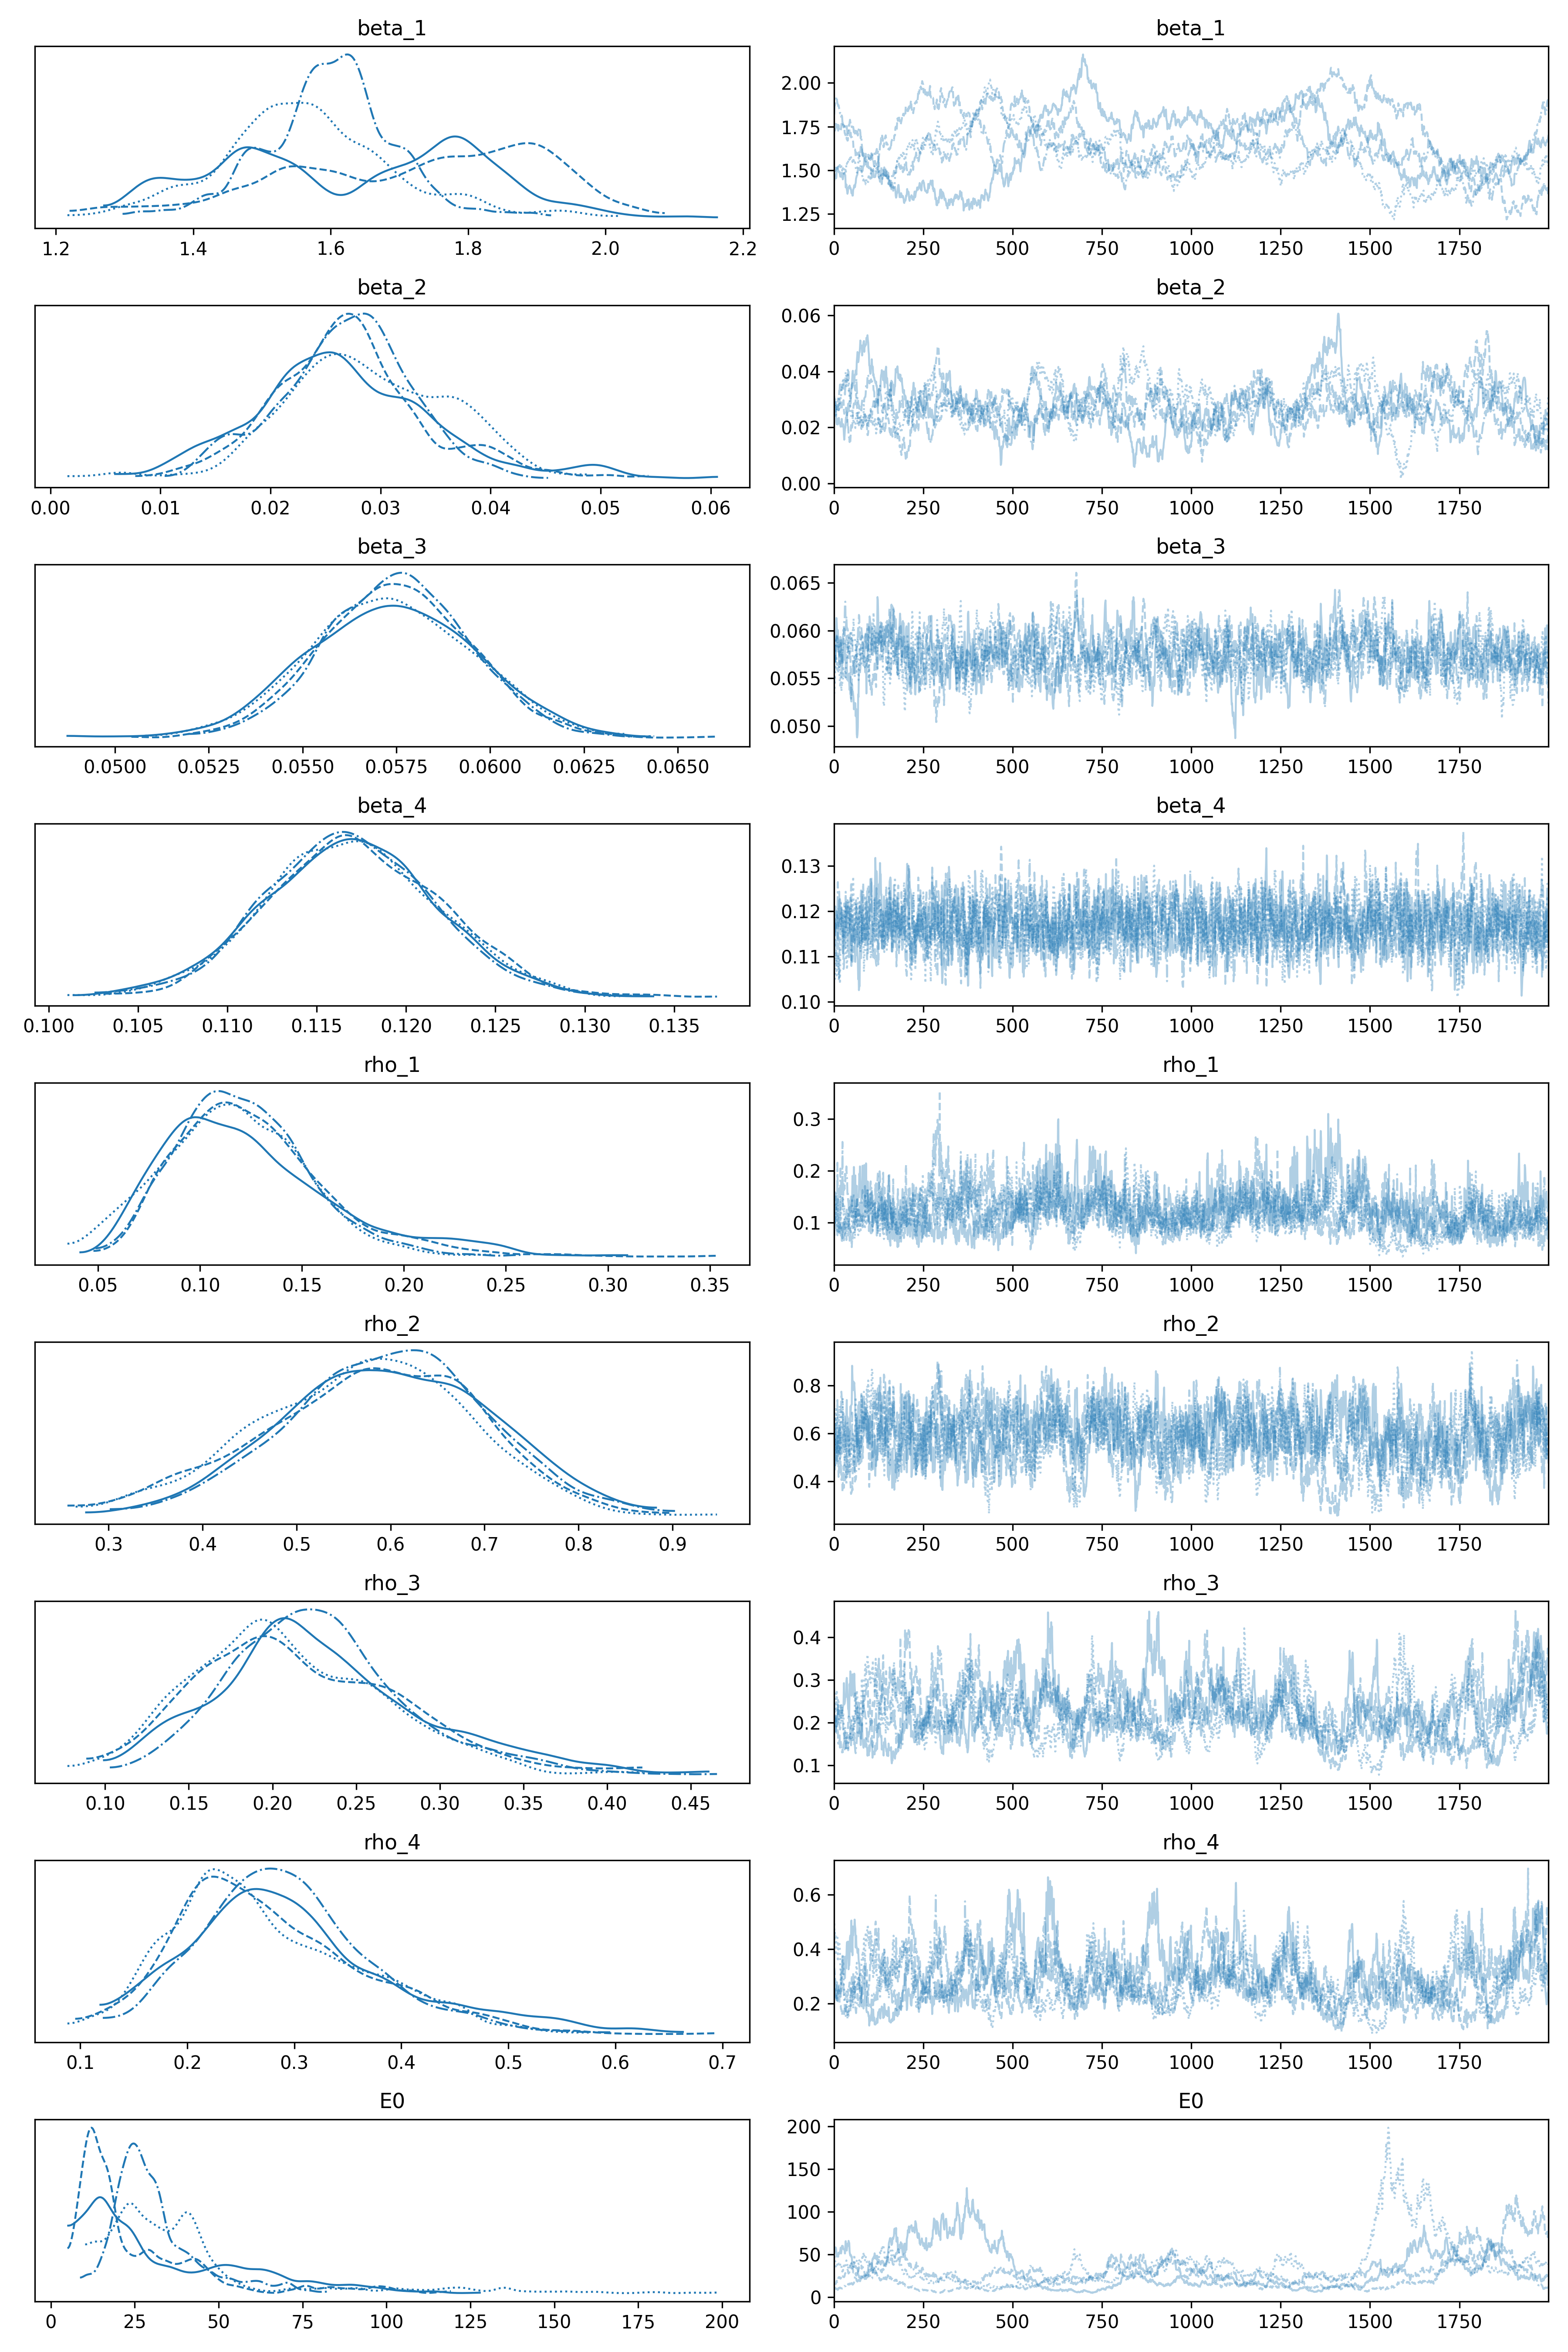
\includegraphics[width=0.90\textwidth]{1/bayesian_trace_plots.png}
    \caption{MCMC trace plots for key model parameters, demonstrating stable convergence of the sampler chains.}
    \label{fig:trace_plots}
\end{figure}

\section{Python Code Listings}

\subsection{Data Processing Script (data\_processing.py)}
\begin{lstlisting}[language=Python, caption=Python script for processing raw OWID data into a clean dataset for Germany.]
import pandas as pd

def process_covid_data(input_path='owid-covid-data.csv', output_path='germany_covid_processed.csv'):
    """
    Loads, filters, cleans, and processes COVID-19 data for Germany for a specific period,
    generating a clean data table for SEIAR model fitting.
    """
    print(f"Starting data processing, reading from '{input_path}'...")

    try:
        # --- 1. Load and Filter ---
        df = pd.read_csv(input_path)

        # Convert 'date' column to datetime objects for easy filtering
        df['date'] = pd.to_datetime(df['date'])

        # a. Filter for location 'Germany'
        df_germany = df[df['location'] == 'Germany'].copy()

        # b. Filter for dates between '2020-03-01' and '2021-03-01'
        start_date = '2020-03-01'
        end_date = '2021-03-01'
        mask = (df_germany['date'] >= start_date) & (df_germany['date'] <= end_date)
        df_processed = df_germany.loc[mask].copy()
        
        print(f"Successfully filtered data for Germany from {start_date} to {end_date}.")

        # --- 2. Data Cleaning and Smoothing ---

        # a. Handle missing values: Fill NaN in 'new_cases' with 0
        df_processed['new_cases'] = df_processed['new_cases'].fillna(0)

        # b. Calculate 7-day moving average to smooth new cases
        df_processed['new_cases_smoothed'] = df_processed['new_cases'].rolling(window=7, center=True).mean()
        # The moving average will create NaNs at the beginning and end of the series, which we need to fill
        # Use forward and backward fill (bfill/ffill) to handle these edge cases
        df_processed['new_cases_smoothed'] = df_processed['new_cases_smoothed'].fillna(method='bfill').fillna(method='ffill')
        
        print("Completed smoothing of new cases (7-day moving average).")

        # --- 3. Calculate Core Fitting Data ---

        # Calculate the estimated current number of infectious individuals (19-day rolling sum)
        infection_period = 19
        df_processed['infectious_pool'] = df_processed['new_cases_smoothed'].rolling(window=infection_period).sum()
        # Similarly, handle NaNs produced at the beginning by the rolling sum
        df_processed['infectious_pool'] = df_processed['infectious_pool'].fillna(0)

        print(f"Completed estimation of the infectious pool ({infection_period}-day rolling sum).")

        # --- 4. Finalize and Save ---
        
        # a. Create a time series column starting from 0
        df_processed.reset_index(drop=True, inplace=True)
        df_processed['time'] = df_processed.index

        # b. Keep only the required columns
        # We also need the 'population' column
        final_columns = ['date', 'time', 'new_cases_smoothed', 'infectious_pool', 'population']
        df_final = df_processed[final_columns].copy()

        # Convert date column back to string format for saving
        df_final['date'] = df_final['date'].dt.strftime('%Y-%m-%d')

        # c. Save to a new CSV file
        df_final.to_csv(output_path, index=False)
        
        print(f"\nProcessing complete! Clean data saved to '{output_path}'.")
        print("Final data contains the following columns:")
        print(df_final.info())
        print("\nData preview:")
        print(df_final.head())
        
        return df_final

    except FileNotFoundError:
        print(f"Error: Input file '{input_path}' not found. Please ensure the file exists.")
        return None
    except Exception as e:
        print(f"An error occurred during processing: {e}")
        return None

if __name__ == '__main__':
    process_covid_data()
\end{lstlisting}

\subsection{Deterministic Two-Stage Model Script (script.py)}
\begin{lstlisting}[language=Python, caption={Python script for fitting a two-stage piecewise deterministic SEIAR model, corresponding to the pre- and post-lockdown phases.}]
import pandas as pd
import numpy as np
from scipy.integrate import odeint
from scipy.optimize import curve_fit
import matplotlib.pyplot as plt

# --- Step 1: Import libraries and load data ---

# Load the processed German epidemic data
try:
    df = pd.read_csv('germany_covid_processed.csv')
    # Core fitting data: estimated total current infectious individuals
    i_data = df['infectious_pool'].values
    t_data = np.arange(len(i_data))
    # Get total population N
    N = df['population'].iloc[0]
except FileNotFoundError:
    print("Error: Data file 'germany_covid_processed.csv' not found.")
    print("Please ensure you have run data_processing.py to generate this file.")
    exit()

# --- Global parameters and initial conditions ---
# Fixed parameters (from literature in Part 2 of our report)
F = 0.17       # Asymptomatic proportion
SIGMA = 1/4.5    # Latent period transition rate (1/day)
GAMMA_I = 1/19.5 # Symptomatic recovery rate (1/day)
GAMMA_A = 1/17.0   # Asymptomatic recovery rate (1/day)

# Initial conditions
I0 = 0      # Assume no diagnosed symptomatic individuals at t=0
A0 = 0      # Assume no asymptomatic individuals at t=0
E0 = 1      # Key: Assume 1 exposed individual enters the population at t=0, as the "seed" of the epidemic
R0 = 0
S0 = N - I0 - E0 - A0 - R0
Y0 = (S0, E0, I0, A0, R0) # Initial state tuple

# --- Step 2: Define the SEIAR model function ---

# Define the differential equations for the SEIAR model
# We take all parameters as inputs to increase the function's versatility
def seiar_model(y, t, N, beta_I, f_param, sigma_param, gamma_i_param, gamma_a_param):
    """
    ODE system for the SEIAR model.
    beta_I is now a parameter, not a global variable.
    """
    S, E, I, A, R = y
    
    # Calculate beta_A based on the relationship from literature
    beta_A = 0.58 * beta_I
    
    # Differential equations
    dSdt = -beta_I * S * I / N - beta_A * S * A / N
    dEdt = beta_I * S * I / N + beta_A * S * A / N - sigma_param * E
    dIdt = (1 - f_param) * sigma_param * E - gamma_i_param * I
    dAdt = f_param * sigma_param * E - gamma_a_param * A
    dRdt = gamma_i_param * I + gamma_a_param * A
    
    return dSdt, dEdt, dIdt, dAdt, dRdt

# --- Step 3: Create a new, more powerful "solver" function ---

def fit_odeint_piecewise(t, beta_pre, beta_post, rho, E0_fit):
    """
    An advanced solver for curve_fit.
    It uses a piecewise-changing beta and simultaneously fits the observation proportion rho and initial exposed count E0.
    """
    t_switch = 22  # Approximate date of Germany's national lockdown (2020-03-22), corresponding to day 22 in the data

    # Update initial conditions with the fitted parameters
    # E0 is to be fitted; I0, A0, R0 start from 0
    y0_fit = (N - E0_fit, E0_fit, 0, 0, 0)

    # Split the time array into "pre-lockdown" and "post-lockdown"
    t_pre = t[t < t_switch]
    t_post = t[t >= t_switch]

    # Create an empty numpy array to store the combined infected population
    infected_combined = np.array([])
    
    # Solve for the first phase (pre-lockdown)
    if len(t_pre) > 0:
        # Solve using the pre-lockdown beta
        res_pre = odeint(seiar_model, y0_fit, t_pre, args=(N, beta_pre, F, SIGMA, GAMMA_I, GAMMA_A))
        # Extract the I+A part
        infected_pre = res_pre[:, 2] + res_pre[:, 3]
        infected_combined = np.concatenate((infected_combined, infected_pre))
        # The initial condition for the second phase is the end point of the first phase
        y0_post = res_pre[-1]
    else:
        # If the fitting window is entirely after the lockdown, the initial condition for the second phase is our specified y0_fit
        y0_post = y0_fit

    # Solve for the second phase (post-lockdown)
    if len(t_post) > 0:
        # Solve using the post-lockdown beta
        res_post = odeint(seiar_model, y0_post, t_post, args=(N, beta_post, F, SIGMA, GAMMA_I, GAMMA_A))
        # Extract the I+A part
        infected_post = res_post[:, 2] + res_post[:, 3]
        infected_combined = np.concatenate((infected_combined, infected_post))

    # Return the model prediction scaled by the observation proportion rho
    return rho * infected_combined

# --- Step 4: Perform the fit and visualize ---

# Define the fitting window
fit_duration = 180
t_fit = t_data[:fit_duration]
i_fit = i_data[:fit_duration]

# Provide initial guesses and bounds for the 4 parameters to be fitted
# Parameter order: [beta_pre, beta_post, rho, E0_fit]
initial_guesses = [0.6, 0.1, 0.2, 100]
bounds = (
    [0.1, 0.01, 0.01, 1],      # Lower bounds
    [2.0, 1.0, 1.0, 50000]     # Upper bounds
)

# Perform the fit
try:
    popt, pcov = curve_fit(
        fit_odeint_piecewise,
        t_fit, 
        i_fit, 
        p0=initial_guesses, 
        bounds=bounds,
        maxfev=3000  # Increase max iterations to help convergence
    )
    
    # Extract optimal parameters
    beta_pre_opt, beta_post_opt, rho_opt, E0_fit_opt = popt
    
    print("Fit successful!")
    print(f"Pre-lockdown transmission rate (beta_pre): {beta_pre_opt:.4f}")
    print(f"Post-lockdown transmission rate (beta_post): {beta_post_opt:.4f}")
    print(f"Case observation proportion (rho): {rho_opt:.4f}")
    print(f"Initial exposed population (E0_fit): {E0_fit_opt:.2f}")

    # --- Visualization ---
    
    # Rerun the solver with optimal parameters to generate the final fitted curve
    fitted_curve = fit_odeint_piecewise(t_fit, *popt)
    
    # Create the plot
    plt.figure(figsize=(14, 9))
    # Plot all real data points (entire time series)
    plt.plot(t_data, i_data, 'o', label='Real Data (Estimated Total Infectious)', markersize=4, alpha=0.5)
    # Plot the fitted curve within the fitting window
    plt.plot(t_fit, fitted_curve, 'r-', label='Fitted SEIAR Model', linewidth=3)
    
    # Mark the lockdown date with a vertical line
    t_switch = 22
    plt.axvline(x=t_switch, color='k', linestyle='--', label=f'Lockdown Start (Day {t_switch})')
    
    # Annotate the plot with the optimal parameter values
    param_text = (
        f'Fitted Parameters:\n'
        f'$\\beta_{{pre}}$ = {beta_pre_opt:.3f}\n'
        f'$\\beta_{{post}}$ = {beta_post_opt:.3f}\n'
        f'$\\rho$ (rho) = {rho_opt:.3f}\n'
        f'$E_0$ = {E0_fit_opt:.0f}'
    )
    plt.text(0.65, 0.7, param_text, transform=plt.gca().transAxes, fontsize=12,
             verticalalignment='top', bbox=dict(boxstyle='round,pad=0.5', fc='wheat', alpha=0.5))
    
    # Format the plot
    plt.title('SEIAR Model with Piecewise Beta Fit to German COVID-19 Data', fontsize=16)
    plt.xlabel('Days Since 2020-03-01', fontsize=12)
    plt.ylabel('Infectious Population', fontsize=12)
    plt.legend(fontsize=11)
    plt.grid(True, which='both', linestyle='--', linewidth=0.5)
    plt.ylim(bottom=0)
    plt.xlim(left=0, right=len(t_data))
    
    # Save the figure
    plt.savefig('seiar_fit_germany_piecewise.png', dpi=300)
    print("\nFit result plot saved as 'seiar_fit_germany_piecewise.png'")
    
    # Display the plot
    plt.show()

except RuntimeError as e:
    print(f"Error: Could not complete the fit. Error message: {e}")
    print("This might be due to poor initial guesses or bounds. Try adjusting `initial_guesses` and `bounds`.")

except Exception as e:
    print(f"An unknown error occurred: {e}")
\end{lstlisting}

\subsection{Deterministic Four-Stage Model Script (script\_piecewise.py)}
\begin{lstlisting}[language=Python, caption={Python script for fitting a four-stage piecewise deterministic SEIAR model, aligning with the Bayesian model's structure.}]
import pandas as pd
import numpy as np
from scipy.integrate import odeint
from scipy.optimize import curve_fit
import matplotlib.pyplot as plt
import matplotlib.dates as mdates

def seiar_model(y, t, beta, N, f, sigma, gamma_i, gamma_a):
    """
    Standard SEIAR model ODE function for use by the internal solver.
    """
    S, E, I, A, R = y
    beta_a = 0.58 * beta  # Asymptomatic transmission rate is a fixed relative proportion
    
    force_of_infection = (beta * I + beta_a * A) * S / N
    
    dSdt = -force_of_infection
    dEdt = force_of_infection - sigma * E
    dIdt = (1 - f) * sigma * E - gamma_i * I
    dAdt = f * sigma * E - gamma_a * A
    dRdt = gamma_i * I + gamma_a * A
    
    return [dSdt, dEdt, dIdt, dAdt, dRdt]

def piecewise_seiar_model(t_data, beta1, beta2, beta3, beta4):
    """
    Piecewise SEIAR model for use with curve_fit.
    This function takes an array of time points and four beta parameters,
    and returns the predicted (I+A) curve for the entire period.
    """
    # Define breakpoints (consistent with the Bayesian model)
    breakpoints = [22, 71, 184]
    betas = [beta1, beta2, beta3, beta4]
    
    # Full time span
    t_full = np.arange(len(t_data))
    
    # Initialize the overall solution
    solution = np.array([]).reshape(0, 5)
    
    # Initial conditions
    # Get an estimate for initial E0 from the data (a small non-zero value)
    # We could also make E0 a fitting parameter, but for simplicity, we use a reasonable estimate here.
    initial_exposed = 500 
    current_y0 = [N - initial_exposed, initial_exposed, 0, 0, 0]
    
    # Solve the ODE segment by segment
    last_t = 0
    for i, bp in enumerate(breakpoints):
        # Define the time array for the current segment
        t_segment = np.arange(last_t, bp)
        
        # Solve the current segment
        sol_segment = odeint(
            seiar_model,
            y0=current_y0,
            t=t_segment,
            args=(betas[i], N, F, SIGMA, GAMMA_I, GAMMA_A)
        )
        
        # Concatenate the solution
        solution = np.vstack([solution, sol_segment])
        
        # Update initial conditions and start time for the next segment
        current_y0 = sol_segment[-1]
        last_t = bp

    # Solve the final segment
    t_segment_final = np.arange(last_t, len(t_full))
    sol_segment_final = odeint(
        seiar_model,
        y0=current_y0,
        t=t_segment_final,
        args=(betas[-1], N, F, SIGMA, GAMMA_I, GAMMA_A)
    )
    
    # Concatenate the final segment's solution
    solution = np.vstack([solution, sol_segment_final])

    # Return the model's predicted total infected population (I+A)
    return solution[:, 2] + solution[:, 3]


# --- 1. Load and prepare data ---
df_data = pd.read_csv('germany_covid_processed.csv', parse_dates=['date'])

# Define model parameters (based on literature)
F = 0.17
SIGMA = 1/4.5
GAMMA_I = 1/19.5
GAMMA_A = 1/17.0
N = df_data['population'].iloc[0]

# Prepare data for fitting (using the first 270 days)
fit_duration = 270
data_to_fit = df_data.head(fit_duration)
y_data = data_to_fit['infectious_pool'].values
x_data = np.arange(len(y_data))
dates = data_to_fit['date']

# --- 2. Perform piecewise deterministic fit ---
print("Performing piecewise deterministic fit...")

# Provide initial guesses and bounds for the four beta parameters
initial_guesses = [0.2, 0.1, 0.15, 0.1]
bounds = (0, [1.0, 1.0, 1.0, 1.0]) # Beta values are typically between 0 and 1

# Call curve_fit
popt, pcov = curve_fit(
    f=piecewise_seiar_model,
    xdata=x_data,
    ydata=y_data,
    p0=initial_guesses,
    bounds=bounds,
    method='trf' # 'trf' is suitable for bounded problems
)

# Extract optimal parameters
beta_opt = popt
print("\nFit complete! Optimal parameters are:")
for i, b in enumerate(beta_opt):
    print(f"  - beta_{i+1}: {b:.4f}")

# --- 3. Generate final fitted curve and plot ---
print("\nGenerating final fit plot...")
# Generate the final model curve using the optimal parameters
model_fit_curve = piecewise_seiar_model(x_data, *beta_opt)

# Plotting
plt.style.use('seaborn-v0_8-whitegrid')
fig, ax = plt.subplots(figsize=(14, 8))

# Plot real data
ax.plot(dates, y_data, 'o', markersize=4, color='dimgray', alpha=0.7, label='Observed Infectious Pool')

# Plot model fit curve
ax.plot(dates, model_fit_curve, color='dodgerblue', linewidth=2.5, label='Piecewise SEIAR Model Fit')

# Add vertical lines and labels for segments
breakpoints_days = [22, 71, 184]
for i, bp_day in enumerate(breakpoints_days):
    bp_date = dates.iloc[0] + pd.to_timedelta(bp_day, unit='D')
    ax.axvline(x=bp_date, linestyle='--', color='gray', linewidth=1.5)
    
# Add parameter labels
bp_dates = [dates.iloc[0]] + [dates.iloc[0] + pd.to_timedelta(d, unit='D') for d in breakpoints_days]
label_positions = [5, 35, 120, 200]
for i, pos in enumerate(label_positions):
     ax.text(dates.iloc[pos], max(y_data)*0.85, f'$\\beta_{i+1}={beta_opt[i]:.3f}$', 
             fontsize=12, backgroundcolor='white', color='blue')

# Format the plot
ax.set_title('Piecewise Deterministic SEIAR Model Fit to German COVID-19 Data', fontsize=16, pad=20)
ax.set_xlabel('Date', fontsize=12)
ax.set_ylabel('Estimated Infectious Population', fontsize=12)
ax.legend(fontsize=11)
ax.grid(True)

# Format date display
ax.xaxis.set_major_locator(mdates.MonthLocator(interval=2))
ax.xaxis.set_major_formatter(mdates.DateFormatter('%Y-%m'))
fig.autofmt_xdate()

# Save the figure
output_filename = 'seiar_fit_germany_piecewise.png'
plt.tight_layout()
plt.savefig(output_filename, dpi=300)

print(f"\nSuccess! Final fit plot saved as '{output_filename}'")
plt.show() 
\end{lstlisting} 

\subsection{Bayesian Model Script (script\_bayesian.py)}
\begin{lstlisting}[language=Python, caption=Python script for constructing and sampling the Bayesian SEIAR model using PyMC.]
import pandas as pd
import numpy as np
import pymc as pm
import arviz as az
import pytensor.tensor as pt
from pytensor.graph.op import Op
from pytensor.graph import Apply
import matplotlib.pyplot as plt

print(f"PyMC Version: {pm.__version__}")
print(f"ArviZ Version: {az.__version__}")

# --- 1. Data Loading and Preparation ---

try:
    df = pd.read_csv('germany_covid_processed.csv', parse_dates=['date'])
    # We will fit the entire first wave and the beginning of the second wave (approx. 9 months)
    fit_duration = 270 
    i_data = df['infectious_pool'].values[:fit_duration]
    t_data = np.arange(fit_duration)
    N = df['population'].iloc[0]
except FileNotFoundError:
    print("Error: Data file 'germany_covid_processed.csv' not found.")
    exit()

# --- 2. Define ODE System (PyTensor version) ---

# Fixed parameters
F = 0.17       # Asymptomatic proportion
SIGMA = 1/4.5    # Latent period transition rate (1/day)
GAMMA_I = 1/19.5 # Symptomatic recovery rate (1/day)
GAMMA_A = 1/17.0   # Asymptomatic recovery rate (1/day)

# This is the standard way to integrate an external ODE solver (like scipy) in PyMC v5+
# We need to wrap scipy's odeint into a PyTensor Op
class OdeintOp(Op):
    def __init__(self, func, t):
        self._func = func
        self._t = t

    def make_node(self, y0, *theta):
        # Inputs: y0 are the initial conditions, theta are the ODE parameters
        y0 = pt.as_tensor_variable(y0)
        theta = [pt.as_tensor_variable(arg) for arg in theta]
        # Output: The solution to the ODE
        out = pt.tensor(dtype=y0.dtype, broadcastable=(False, False))
        return Apply(self, [y0] + theta, [out])

    def perform(self, node, inputs, output_storage):
        from scipy.integrate import odeint
        y0 = inputs[0]
        theta = inputs[1:]
        # odeint requires a function that only accepts (y, t, *args)
        def grad_func(y, t, *args):
            return self._func(y, t, *args)
        # Solve the ODE
        result = odeint(grad_func, y0, self._t, args=tuple(theta))
        output_storage[0][0] = result.astype(y0.dtype)

# The SEIAR model's differential equations, now usable by OdeintOp
def seiar_model_scipy(y, t, beta):
    S, E, I, A, R = y
    # According to literature, the transmission rate of asymptomatic individuals is 0.58 times that of symptomatic ones
    beta_A = 0.58 * beta
    
    # Correct force of infection calculation
    force_of_infection = (beta * I + beta_A * A) * S / N
    
    dSdt = -force_of_infection
    dEdt = force_of_infection - SIGMA * E
    dIdt = (1 - F) * SIGMA * E - GAMMA_I * I
    dAdt = F * SIGMA * E - GAMMA_A * A
    dRdt = GAMMA_I * I + GAMMA_A * A
    
    return [dSdt, dEdt, dIdt, dAdt, dRdt]


# --- 3. Build PyMC Bayesian Model ---

# Define piecewise time points (based on your suggestion)
# Add a new breakpoint in early September (around day 184)
# Segment 1: 0-21, Segment 2: 22-70, Segment 3: 71-183, Segment 4: 184-269
breakpoints = [22, 71, 184]
t_segs = [
    np.arange(0, breakpoints[0]),
    np.arange(breakpoints[0], breakpoints[1]),
    np.arange(breakpoints[1], breakpoints[2]),
    np.arange(breakpoints[2], fit_duration)
]

with pm.Model() as model:
    # --- Priors ---
    
    # 1. Transmission rate beta (in four segments)
    # beta_1 uses a strong prior based on R0 knowledge
    beta_1 = pm.Gamma('beta_1', alpha=10, beta=50) # mean 0.2, R0 approx 3.5, strong constraint
    # Priors for beta_2, beta_3, beta_4 are more lenient
    beta_2 = pm.Gamma('beta_2', alpha=2, beta=4) # mean 0.5
    beta_3 = pm.Gamma('beta_3', alpha=2, beta=4) # mean 0.5
    beta_4 = pm.Gamma('beta_4', alpha=2, beta=4) # Prior for the new segment
    betas = [beta_1, beta_2, beta_3, beta_4]
    
    # 2. Observation proportion rho (in four segments)
    rho_1 = pm.Beta('rho_1', alpha=2, beta=8) # Prior assumes a lower proportion
    rho_2 = pm.Beta('rho_2', alpha=4, beta=6) # After lockdown, testing capacity increased, so proportion might be slightly higher
    rho_3 = pm.Beta('rho_3', alpha=4, beta=6)
    rho_4 = pm.Beta('rho_4', alpha=4, beta=6) # Prior for the new segment
    
    # Use pytensor.switch to implement piecewise rho (rho is not in the ODE itself, but used during observation)
    rho_t = pt.switch(t_data < breakpoints[0], rho_1,
                      pt.switch(t_data < breakpoints[1], rho_2,
                                pt.switch(t_data < breakpoints[2], rho_3, rho_4)))
                      
    # 3. Initial exposed population E0 - Using a Gamma prior for better stability
    E0 = pm.Gamma('E0', alpha=2, beta=1/250) # mean 500
    
    # 4. Observation noise (for the Negative Binomial distribution)
    # The larger alpha, the closer the distribution is to Poisson (variance=mean); the smaller alpha, the larger the variance (overdispersion)
    noise_alpha = pm.Exponential('noise_alpha', 1.0)

    # --- Piecewise ODE Solving ---
    y0 = pt.stack([N - E0, E0, 0, 0, 0])
    
    all_sols = []
    current_y0 = y0

    for i, t_seg in enumerate(t_segs):
        # Create an ODE solver instance for each segment
        ode_solver_seg = OdeintOp(seiar_model_scipy, t_seg)
        # Solve using the corresponding beta
        sol_seg = ode_solver_seg(current_y0, betas[i])
        
        # Add the solution of the current segment to the list
        all_sols.append(sol_seg)
        
        # Update the initial conditions for the next segment
        # We need to ensure this is a valid operation in the Theano/PyTensor computation graph
        # sol_seg[-1] will take the state at the last time point
        current_y0 = sol_seg[-1]

    # Concatenate the solutions from all segments
    ode_solutions = pt.concatenate(all_sols, axis=0)
    
    # Extract the model's predicted I and A
    I_model = ode_solutions[:, 2]
    A_model = ode_solutions[:, 3]
    
    # Calculate the model's predicted "observable" cases
    # Here we use the piecewise rho_t to adjust the output
    mu = rho_t * (I_model + A_model)

    # --- Likelihood ---
    
    # We use a Negative Binomial distribution, which handles overdispersion in epidemic data better than Poisson
    pm.NegativeBinomial('obs', mu=mu + 1e-6, alpha=noise_alpha, observed=i_data)


# --- 4. Run MCMC Sampling ---

if __name__ == "__main__":
    with model:
        print("Starting MCMC sampling... This might take a few minutes...")
        # The JAX sampler is usually faster
        try:
            idata = pm.sample(2000, tune=1000, chains=4, cores=1, target_accept=0.9, nuts_sampler="numpyro")
        except Exception:
            print("Numpyro sampling failed, switching to the default NUTS sampler...")
            idata = pm.sample(2000, tune=1000, chains=4, cores=1, target_accept=0.9)

    # --- 5. Results Analysis and Visualization ---
    
    # Print the posterior statistics summary for the parameters
    summary = az.summary(idata, var_names=['beta_1', 'beta_2', 'beta_3', 'beta_4', 'rho_1', 'rho_2', 'rho_3', 'rho_4', 'E0', 'noise_alpha'])
    print("\n--- Parameter Posterior Distribution Summary ---")
    print(summary)
    
    # Save summary to CSV
    summary.to_csv("bayesian_summary.csv")
    print("\nSummary saved to 'bayesian_summary.csv'")

    # Plot posterior distribution plots
    try:
        print("\nGenerating posterior distribution plots...")
        az.plot_posterior(idata, var_names=['beta_1', 'beta_2', 'beta_3', 'beta_4', 'rho_1', 'rho_2', 'rho_3', 'rho_4', 'E0'])
        plt.tight_layout()
        plt.savefig("bayesian_posterior_plots.png", dpi=300)
        print("Posterior distribution plots saved as 'bayesian_posterior_plots.png'")
        plt.show()
    except Exception as e:
        print(f"Could not generate posterior plots: {e}")

    # Plot trace plots (for diagnostics)
    try:
        print("\nGenerating trace plots...")
        az.plot_trace(idata, var_names=['beta_1', 'beta_2', 'beta_3', 'beta_4', 'rho_1', 'rho_2', 'rho_3', 'rho_4', 'E0'])
        plt.tight_layout()
        plt.savefig("bayesian_trace_plots.png", dpi=300)
        print("Trace plots saved as 'bayesian_trace_plots.png'")
        plt.show()
    except Exception as e:
        print(f"Could not generate trace plots: {e}")
\end{lstlisting}

\subsection{Plotting and Scenario Analysis Script (plot\_bayesian\_results.py)}
\begin{lstlisting}[language=Python, caption=Python script for plotting the Bayesian model fit and running the scenario analysis.]
import pandas as pd
import numpy as np
from scipy.integrate import odeint
import matplotlib.pyplot as plt
import matplotlib.dates as mdates

# It's good practice to handle the minus sign display in plots
plt.rcParams['axes.unicode_minus'] = False

def seiar_model_scipy(y, t, beta, N, F, SIGMA, GAMMA_I, GAMMA_A):
    """
    SEIAR ODE model function for use with scipy.integrate.odeint.
    """
    S, E, I, A, R = y
    beta_A = 0.58 * beta
    
    force_of_infection = (beta * I + beta_A * A) * S / N
    
    dSdt = -force_of_infection
    dEdt = force_of_infection - SIGMA * E
    dIdt = (1 - F) * SIGMA * E - GAMMA_I * I
    dAdt = F * SIGMA * E - GAMMA_A * A
    dRdt = GAMMA_I * I + GAMMA_A * A
    
    return [dSdt, dEdt, dIdt, dAdt, dRdt]

def plot_results():
    """
    Main function to load data and results, and generate the final fit plot.
    """
    # --- 1. Load Data and Parameters ---
    try:
        df_data = pd.read_csv('germany_covid_processed.csv', parse_dates=['date'])
        df_summary = pd.read_csv('bayesian_summary.csv', index_col=0)
    except FileNotFoundError as e:
        print(f"Error: Missing required file: {e.filename}")
        print("Please ensure 'germany_covid_processed.csv' and 'bayesian_summary.csv' are in the current directory.")
        return

    # Extract posterior means as our point estimate parameters
    params = df_summary['mean']
    beta_1, beta_2, beta_3, beta_4 = params['beta_1'], params['beta_2'], params['beta_3'], params['beta_4']
    rho_1, rho_2, rho_3, rho_4 = params['rho_1'], params['rho_2'], params['rho_3'], params['rho_4']
    E0 = params['E0']
    
    # Fixed model parameters
    F = 0.17
    SIGMA = 1/4.5
    GAMMA_I = 1/19.5
    GAMMA_A = 1/17.0
    N = df_data['population'].iloc[0]

    # Prepare data required for fitting
    fit_duration = 270
    dates = df_data['date'].iloc[:fit_duration]
    i_data = df_data['infectious_pool'].values[:fit_duration]

    # --- 2. Solve ODE Piecewise Using Extracted Parameters ---
    
    # Define breakpoints and time arrays
    breakpoints = [22, 71, 184]
    t_segs = [
        np.arange(0, breakpoints[0]),
        np.arange(breakpoints[0], breakpoints[1]),
        np.arange(breakpoints[1], breakpoints[2]),
        np.arange(breakpoints[2], fit_duration)
    ]
    betas = [beta_1, beta_2, beta_3, beta_4]
    
    # Initial conditions
    y0 = [N - E0, E0, 0, 0, 0]
    
    all_solutions = []
    current_y0 = y0
    
    # Loop to solve each segment
    for i, t_seg in enumerate(t_segs):
        sol = odeint(
            seiar_model_scipy,
            y0=current_y0,
            t=t_seg,
            args=(betas[i], N, F, SIGMA, GAMMA_I, GAMMA_A)
        )
        all_solutions.append(sol)
        # The initial condition for the next segment is the final state of the current one
        current_y0 = sol[-1]
        
    # Concatenate all solutions
    model_output = np.concatenate(all_solutions, axis=0)
    I_model = model_output[:, 2]
    A_model = model_output[:, 3]
    
    # --- 3. Calculate Observable Cases (mu) ---
    t_full = np.arange(fit_duration)
    # Construct piecewise rho values based on breakpoints
    # Use more direct boolean indexing to build piecewise rho for clarity and robustness
    rho_t = np.zeros(fit_duration)
    rho_t[t_full < breakpoints[0]] = rho_1
    rho_t[(t_full >= breakpoints[0]) & (t_full < breakpoints[1])] = rho_2
    rho_t[(t_full >= breakpoints[1]) & (t_full < breakpoints[2])] = rho_3
    rho_t[t_full >= breakpoints[2]] = rho_4
                         
    # This is the model's predicted daily infectious count, comparable to the real data
    mu_predicted = rho_t * (I_model + A_model)

    # --- 4. Plotting ---
    print("Generating final fit plot...")
    plt.style.use('seaborn-v0_8-whitegrid')
    fig, ax = plt.subplots(figsize=(14, 8))
    
    # Plot real data
    ax.plot(dates, i_data, 'o', markersize=4, color='dimgray', alpha=0.7, label='Observed Data (7-day smoothed)')
    
    # Plot model fit curve
    ax.plot(dates, mu_predicted, color='crimson', linewidth=2.5, label='SEIAR Model Prediction (Mean Posterior)')
    
    # Add vertical lines and labels for segments
    for bp_day in breakpoints:
        bp_date = dates.iloc[0] + pd.to_timedelta(bp_day, unit='D')
        ax.axvline(x=bp_date, linestyle='--', color='gray', linewidth=1.5)

    ax.text(dates.iloc[5], max(i_data)*0.8, f'$\\beta_1={beta_1:.3f}$\n$\\rho_1={rho_1:.3f}$', fontsize=12, backgroundcolor='white')
    ax.text(dates.iloc[35], max(i_data)*0.8, f'$\\beta_2={beta_2:.3f}$\n$\\rho_2={rho_2:.3f}$', fontsize=12, backgroundcolor='white')
    ax.text(dates.iloc[120], max(i_data)*0.8, f'$\\beta_3={beta_3:.3f}$\n$\\rho_3={rho_3:.3f}$', fontsize=12, backgroundcolor='white')
    ax.text(dates.iloc[200], max(i_data)*0.6, f'$\\beta_4={beta_4:.3f}$\n$\\rho_4={rho_4:.3f}$', fontsize=12, backgroundcolor='white')

    # Format the plot
    ax.set_title('Bayesian SEIAR Model Fit to German COVID-19 Data (4 Segments)', fontsize=18, pad=20)
    ax.set_xlabel('Date', fontsize=14)
    ax.set_ylabel('Estimated Infectious Population', fontsize=14)
    ax.legend(fontsize=12)
    ax.grid(True)
    
    # Format date display
    ax.xaxis.set_major_locator(mdates.MonthLocator())
    ax.xaxis.set_major_formatter(mdates.DateFormatter('%Y-%m'))
    fig.autofmt_xdate()
    
    plt.tight_layout()
    plt.savefig('bayesian_fit_to_data.png', dpi=300)
    print("Success! Final fit plot saved as 'bayesian_fit_to_data.png'")
    plt.show()

def run_scenario_analysis():
    """
    Runs and visualizes the scenario analysis, comparing baseline and intervention effects.
    """
    print("\n--- Starting Scenario Analysis ---")

    # --- 1. Get Baseline Parameters ---
    try:
        summary = pd.read_csv("bayesian_summary.csv", index_col=0)
        beta_baseline = summary.loc['beta_1']['mean']
        E0_baseline = summary.loc['E0']['mean']
        
        # Get other fixed parameters from the previous run
        df_data = pd.read_csv('germany_covid_processed.csv', parse_dates=['date'])
        F = 0.17
        SIGMA = 1/4.5
        GAMMA_I = 1/19.5
        GAMMA_A = 1/17.0
        N = df_data['population'].iloc[0]
        
        print(f"Using baseline parameters: beta_1 = {beta_baseline:.4f}, E0 = {E0_baseline:.2f}")

    except Exception as e:
        print(f"Could not read MCMC summary or data file. Using example values. Error: {e}")
        # If file reading fails, use some reasonable approximations and default values
        beta_baseline = 0.4 
        E0_baseline = 500
        N = 83000000
        F = 0.17
        SIGMA = 1/4.5
        GAMMA_I = 1/19.5
        GAMMA_A = 1/17.0

    # --- 2. Simulate Scenarios ---
    beta_intervention = 0.8 * beta_baseline
    t_scenario = np.arange(365) 
    y0_scenario = (N - E0_baseline, E0_baseline, 0, 0, 0)

    # Prepare argument tuple for odeint
    args_baseline = (beta_baseline, N, F, SIGMA, GAMMA_I, GAMMA_A)
    args_intervention = (beta_intervention, N, F, SIGMA, GAMMA_I, GAMMA_A)

    # Run baseline scenario simulation
    ret_baseline = odeint(seiar_model_scipy, y0_scenario, t_scenario, args=args_baseline)
    infected_baseline = ret_baseline[:, 2] + ret_baseline[:, 3]

    # Run intervention scenario simulation
    ret_intervention = odeint(seiar_model_scipy, y0_scenario, t_scenario, args=args_intervention)
    infected_intervention = ret_intervention[:, 2] + ret_intervention[:, 3]

    # --- 3. Visualize Scenario Comparison ---
    plt.figure(figsize=(12, 8))
    plt.plot(t_scenario, infected_baseline, 'b-', label=f'Baseline Scenario (β = {beta_baseline:.3f})', linewidth=2)
    plt.plot(t_scenario, infected_intervention, 'g--', label=f'Intervention Scenario (β reduced by 20%)', linewidth=2)

    # Calculate and label peaks
    peak_baseline_val = np.max(infected_baseline)
    peak_baseline_day = np.argmax(infected_baseline)
    peak_intervention_val = np.max(infected_intervention)
    peak_intervention_day = np.argmax(infected_intervention)

    # Annotate peak information on the plot
    plt.plot(peak_baseline_day, peak_baseline_val, 'bo', markersize=8)
    plt.text(peak_baseline_day, peak_baseline_val*1.05, f'Peak: {peak_baseline_val:,.0f} cases\non Day {peak_baseline_day}', color='b', ha='center')
    plt.plot(peak_intervention_day, peak_intervention_val, 'go', markersize=8)
    plt.text(peak_intervention_day, peak_intervention_val*1.05, f'Peak: {peak_intervention_val:,.0f} cases\non Day {peak_intervention_day}', color='g', ha='center')

    # Format the plot
    plt.title('Scenario Analysis: Impact of a 20% Reduction in Transmission Rate', fontsize=16)
    plt.xlabel('Days Since Initial Outbreak', fontsize=12)
    plt.ylabel('Active Infectious Population (I+A)', fontsize=12)
    plt.legend(fontsize=11)
    plt.grid(True, which='both', linestyle='--', linewidth=0.5)
    plt.ylim(bottom=0)

    # Save the figure with the name needed for our LaTeX document
    plt.savefig('1/scenario_simulation.png', dpi=300)
    print("\nScenario analysis plot saved as '1/scenario_simulation.png'")

    # Display the plot
    plt.show()


if __name__ == "__main__":
    plot_results()
    run_scenario_analysis() 
\end{lstlisting}

\section{Data Sources (Click to view with Acrobat Reader)}
\begin{itemize}
    \item \href{run:owid-covid-data.csv}{\textbf{owid-covid-data.csv}}: The raw data file downloaded from Our World in Data. This large file contains global COVID-19 statistics and was used as the primary input for the data processing script.
    \item \href{run:germany_covid_processed.csv}{\textbf{germany\_covid\_processed.csv}}: A processed data file generated by \texttt{data\_processing.py}. It contains the filtered, smoothed, and prepared time series data for Germany, which served as the basis for all model fitting.
    \item \href{run:bayesian_summary.csv}{\textbf{bayesian\_summary.csv}}: The output file from the Bayesian MCMC simulation, generated by \texttt{script\_bayesian.py}. It contains the statistical summary (mean, standard deviation, credible intervals, etc.) for the posterior distributions of all inferred parameters.
\end{itemize}


\end{document}
% ===================================================================
%   文档结束 (Document Ends)
% ===================================================================